%%%%%%%%%%%%%%%%%%%% CVC 2027 submission (Springer LNNS, svproc) %%%%%%%%%%%%%%%%%%%%
% Condensed from paper/draft/MedMamba-SS-TRM_manuscript_v18.md (+ supplement) to the
% SAI/CVC guidelines: <= 18 pages main text, <= 7 pages appendix, references excluded;
% 150-250-word abstract; double-blind (no authors, affiliations or acknowledgments).
% Figures: paper/cvc2027/figures/, re-rendered at LNNS width by make_figures_lnns.py.
% Bibliography order = order of first citation, written by build_bibliography.py
% (run it after moving or adding \cite commands).
% Build (host TeX via Flatpak):
%   flatpak-spawn --host tectonic -X compile --keep-logs <abs path>/main.tex

\documentclass{svproc}

\usepackage{url}
\def\UrlFont{\rmfamily}
\usepackage{graphicx}
\usepackage{float}
\usepackage{placeins}
\usepackage{amsmath,amssymb}
\usepackage{booktabs}
\usepackage{array}
\usepackage{cite}
\usepackage{algorithm}
\usepackage{algpseudocode}
\usepackage{tikz}
\usetikzlibrary{arrows.meta,positioning}
\graphicspath{{figures/}}
\emergencystretch=1.5em

\newcolumntype{L}[1]{>{\raggedright\arraybackslash}p{#1}}
\newcommand{\ms}{\ensuremath{\,\pm\,}}   % mean +- s.d. in running text
\newcommand{\pt}{\ensuremath{\pm}}       % the same, tight, inside tables
\newcommand{\sd}[1]{{\tiny\ensuremath{\pm}#1}}  % small s.d. inside wide tables

% colour code of the architecture diagram
\definecolor{inheritc}{HTML}{E8EAED}
\definecolor{changedc}{HTML}{FDE68A}
\definecolor{newc}{HTML}{BBF7D0}
\definecolor{trmc}{HTML}{BFDBFE}
\definecolor{removedc}{HTML}{FEE2E2}
\tikzset{
  blk/.style={draw, rounded corners=2pt, align=center, font=\scriptsize,
              minimum height=8.5mm, inner sep=2pt, text width=#1},
  blk/.default=17mm,
  inh/.style={blk, fill=inheritc, draw=gray!70!black},
  chg/.style={blk, fill=changedc, draw=orange!70!black, thick},
  nw/.style={blk, fill=newc, draw=green!50!black, thick},
  trm/.style={blk, fill=trmc, draw=blue!70!black, thick},
  rem/.style={blk, fill=removedc, draw=red!70!black, thick, dashed},
  arr/.style={-{Stealth[length=2mm]}, semithick},
}

\begin{document}
\mainmatter

\title{MedMamba-SS and MedMamba-SS-TRM: Band-Count-Agnostic Spectral--Spatial Medical Image Classification with a Weight-Shared Recursive Backbone}
\titlerunning{Band-Count-Agnostic Recursive MedMamba}

% Double-blind review: no author names, affiliations or country (CVC 2027 guidelines).
\author{Gabriel Del Valle, Saad Ahmed}
\institute{Lakehead University}

\maketitle

\begin{abstract}
Hyperspectral images carry many narrow bands, but MedMamba, a state-space medical image classifier, embeds its input with a convolution sized by the channel count and blind to wavelength. We extend it twice. MedMamba-SS replaces the patch embedding with a spectral pathway (a wavelength-encoded tokenizer shared across bands, a bidirectional spectral selective scan and band pooling) whose parameters do not depend on the band count, and conditions every stage of the hierarchy on it. MedMamba-SS-TRM replaces that hierarchy with one two-layer core applied recursively, following the Tiny Recursive Model. On breast histology from 45 patients, MedMamba-SS-TRM has 446,409 parameters at both 32 and 3 bands; retrained at eight bands, it keeps 96\,\% of its balanced accuracy (one run), and one checkpoint transfers zero-shot to 16 bands (90.9\,\%) with its encoding scale held fixed. On the five test patients it reaches 92.8\ms1.9\,\% balanced accuracy over five seeds, ahead of single-run MedMamba (own recipe) and, at four and five of five paired seeds, of untuned HybridSN and SpectralFormer; pooled over ten held-out patients, HybridSN leads it at every seed (87.1\,\% against 84.5\,\%). The benefit of 32 over 3 bands is patient-dependent: +4.1 points on test, $-$5.8 on validation ($-$1.9 without one patient). Because the 32 bands were selected with labels that included held-out patients, these hyperspectral results are provisional. The recursive model is 6.2 times smaller than the hierarchy it replaces but needs 22.3 times more arithmetic. MedMamba-SS trains on skin-lesion photographs but not on hyperspectral patches.
\keywords{Hyperspectral imaging, State-space models, Band-count agnosticism, Recursive networks, Weight sharing, Breast histopathology}
\end{abstract}

%======================================================================
\section{Introduction}
%======================================================================
Distinguishing ductal carcinoma \emph{in situ} (DCIS) from invasive ductal carcinoma (IDC) and from healthy breast tissue is a routine histopathological decision made on morphology. Hyperspectral imaging (HSI) adds a physically different measurement: each pixel carries a spectrum of tens to hundreds of narrow bands, and absorption in stained tissue depends on its molecular composition. A classifier that exploits this must read the spectral axis as an ordered physical quantity and, because instruments sample different numbers of bands, should not have to be redesigned for every sensor.

We build on two published architectures. \textbf{MedMamba}~\cite{medmamba} brought selective state-space models to medical image classification: its SS-Conv-SSM block pairs a convolutional branch with a two-dimensional selective scan at linear cost, and a four-stage hierarchy of these blocks was evaluated on sixteen datasets. Its first layer is a strided convolution with a weight for every input channel, so its parameter count is tied to the sensor and band order and wavelength are invisible to it. The \textbf{Tiny Recursive Model} (TRM)~\cite{trm} showed that one two-layer network, applied recursively to an answer state and a latent state, can outperform networks with several times its parameters on reasoning puzzles. Depth from reused weights suits medical HSI, where cohorts are small, annotations scarce~\cite{lu2014,pandey2026} and computational cost and generalization across acquisition conditions open problems~\cite{fatima2025}; but TRM was evaluated on small grids with exact answers, without its arithmetic cost.

We extend these models in two steps, each substituting exactly one component (Fig.~\ref{fig:arch}). \textbf{MedMamba-SS} (spectral--spatial) replaces MedMamba's convolutional patch embedding with a spectral pathway in which no parameter shape depends on the number of bands, and conditions every stage of the inherited hierarchy on its output. \textbf{MedMamba-SS-TRM} then replaces the hierarchy with one weight-shared two-layer core applied recursively under TRM's schedule, keeping the spectral pathway and the classification interface. Channel-adaptive models with the first property exist for microscopy, remote sensing, natural and spectral images~\cite{channelvit,dofa,batformer,carl}; we build such a front end into a medical state-space classifier and evaluate it on hyperspectral histopathology.

We ask whether a model derived from MedMamba can be made independent of the number of bands, in its parameters and its behaviour; whether one recursive core can replace the hierarchy, at what arithmetic cost; and whether HSI input beats an RGB rendering of the same captures when model, recipe, patient split and patch locations are held fixed. The contributions are the two models:
\begin{enumerate}
\item \textbf{MedMamba-SS} (Sect.~\ref{sec:ss}): a spectral pathway that encodes each band's wavelength, models the ordered band sequence with a shared tokenizer, spectral convolutions and a bidirectional selective scan, and pools the band axis away, so that none of its parameters depends on the band count (Proposition~\ref{prop:agnostic}); FiLM conditioning~\cite{film} carries it into every stage. Inside MedMamba-SS-TRM, which shares it, the pathway gives identical parameter counts at 32 and 3 bands and transfers zero-shot to 16 bands with its encoding scale fixed; the hierarchical MedMamba-SS itself trains on skin-lesion photographs but not on hyperspectral patches.
\item \textbf{MedMamba-SS-TRM} (Sect.~\ref{sec:sstrm}): one two-layer core, applied 63 times per forward pass, replaces the hierarchy; the model is 6.2 times smaller than MedMamba-SS and 8.2 times smaller than MedMamba, and has the highest test balanced accuracy at four of five seeds but trails HybridSN pooled over all held-out patients. An analytic cost model shows that weight sharing trades storage for compute: 22.3 times the arithmetic of the hierarchy it replaces.
\end{enumerate}

\begin{figure}[t]
\centering
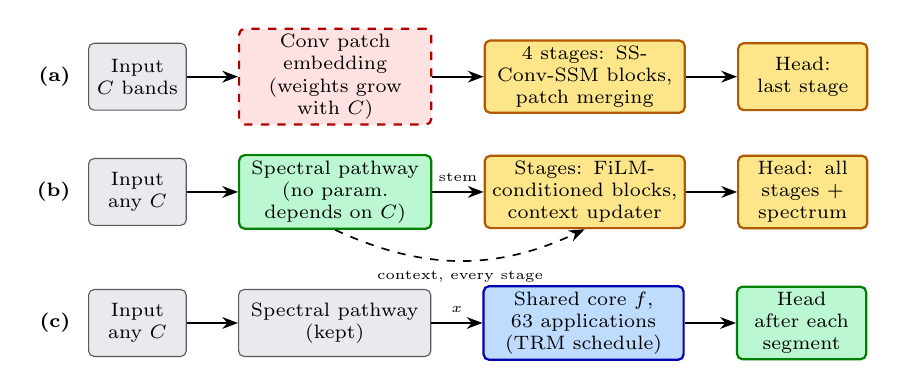
\begin{tikzpicture}[node distance=2.5mm and 6.5mm]
\node[inh, blk=11mm] (aIn) {Input\\$C$ bands};
\node[rem, right=of aIn, blk=23mm] (aEmb) {Conv patch embedding\\(weights grow with $C$)};
\node[chg, right=of aEmb, blk=24mm] (aStg) {4 stages: SS-Conv-SSM blocks, patch merging};
\node[chg, right=of aStg, blk=15mm] (aHd) {Head: last stage};
\draw[arr] (aIn) -- (aEmb); \draw[arr] (aEmb) -- (aStg); \draw[arr] (aStg) -- (aHd);
\node[font=\scriptsize\bfseries, anchor=east] at ([xshift=-1mm]aIn.west) {(a)};
\node[inh, below=6mm of aIn, blk=11mm] (bIn) {Input\\any $C$};
\node[nw, right=of bIn, blk=23mm] (bSp) {Spectral pathway (no param.\ depends on $C$)};
\node[chg, right=of bSp, blk=24mm] (bStg) {Stages: FiLM-conditioned blocks, context updater};
\node[chg, right=of bStg, blk=15mm] (bHd) {Head: all stages + spectrum};
\draw[arr] (bIn) -- (bSp); \draw[arr] (bSp) -- node[above, font=\tiny]{stem} (bStg); \draw[arr] (bStg) -- (bHd);
\draw[arr, dashed] (bSp.south) to[bend right=25] node[below, font=\tiny]{context, every stage} (bStg.south);
\node[font=\scriptsize\bfseries, anchor=east] at ([xshift=-1mm]bIn.west) {(b)};
\node[inh, below=8mm of bIn, blk=11mm] (cIn) {Input\\any $C$};
\node[inh, right=of cIn, blk=23mm] (cSp) {Spectral pathway\\(kept)};
\node[trm, right=of cSp, blk=24mm] (cCore) {Shared core $f$, 63 applications (TRM schedule)};
\node[nw, right=of cCore, blk=15mm] (cHd) {Head after each segment};
\draw[arr] (cIn) -- (cSp); \draw[arr] (cSp) -- node[above, font=\tiny]{$x$} (cCore); \draw[arr] (cCore) -- (cHd);
\node[font=\scriptsize\bfseries, anchor=east] at ([xshift=-1mm]cIn.west) {(c)};
\end{tikzpicture}
\caption{(a) MedMamba~\cite{medmamba}, (b) MedMamba-SS, (c) MedMamba-SS-TRM. Grey: inherited; amber: inherited, modified; green: new; blue: from TRM~\cite{trm}; red dashed: replaced}
\label{fig:arch}
\end{figure}

%======================================================================
\section{Related Work}
%======================================================================
\subsection{State-Space and Recursive Networks}
Residual convolutional networks~\cite{resnet,convnext}, Vision Transformers~\cite{vit} and Swin~\cite{swin} all treat input channels as an unordered set in their first layer. Mamba made state-space parameters input-dependent, giving near-linear sequence modelling~\cite{mamba}; Vision Mamba~\cite{vim} and VMamba~\cite{vmamba} extended it to images, VMamba's two-dimensional selective scan (SS2D) traversing a feature map in four directions, and MedMamba~\cite{medmamba} combined SS2D with a convolutional branch. State-space models have also been applied to the spectral axis: the BiSpectral Mamba module of~\cite{khan2026} scans hyperspectral feature maps in both directions for crop-field classification, and MelanoSpec-SSM diagnoses melanoma against pigmented nevus from hyperspectral pathology images (100 patients, 125 bands between 400 and 1000~nm) at patient level~\cite{melanospec}. Universal Transformers~\cite{ut}, ALBERT~\cite{albert} and deep equilibrium models~\cite{deq} reuse one block in place of many, and Adaptive Computation Time~\cite{act} learns when to stop. TRM~\cite{trm} simplifies the Hierarchical Reasoning Model (HRM)~\cite{hrm} to one two-layer network with two carried states and deep supervision; with 5--7~M parameters it improves on HRM's 27~M on Sudoku-Extreme (87.4\,\% against 55.0\,\%), Maze-Hard and ARC-AGI.

\subsection{Hyperspectral Image Classification}
HybridSN combines 3-D and 2-D convolutions~\cite{hybridsn}, and SpectralFormer embeds groups of neighbouring bands as Transformer tokens~\cite{spectralformer}; both have band-count-dependent parameters and were evaluated on remote-sensing scenes with training and test pixels from the same scene. QuantFormer encodes spectral tokens with a variational quantum circuit at about 35,000 parameters~\cite{quantformer}. Medical HSI is a smaller literature~\cite{lu2014} with scarce annotations, which has motivated label-efficient methods such as SLIC-derived pseudo-labels for hyperspectral melanoma segmentation~\cite{pandey2026}. Histology models also degrade under acquisition shifts such as new magnifications~\cite{fatima2026}; a change of hyperspectral sensor is the spectral counterpart. Ortega et al.\ compared HSI with RGB synthesized from the same cubes under patient-independent partitions and found HSI more accurate for glioblastoma~\cite{ortega2020gbm}, and slightly ahead for breast cancer on 112 images from two patients (test AUC 0.90 against 0.88)~\cite{ortega2020breast}.

\subsection{Band-Count-Agnostic and Channel-Adaptive Models}
ChannelViT builds patch tokens from each channel separately, with a learnable per-channel embedding and hierarchical channel sampling~\cite{channelvit}. DOFA generates patch-embedding weights from each band's wavelength with a hypernetwork~\cite{dofa}. BAT-Former encodes each band separately and fuses the band embeddings, serving RGB images and the HyperLeaf2024 hyperspectral dataset with one model~\cite{batformer}. CARL gives each channel a wavelength encoding and distils any number of channels into a fixed set of spectral tokens by attention; its medical task is porcine organ segmentation from a 100-channel camera~\cite{carl}. Foundation models such as SpectralGPT~\cite{spectralgpt} and HyperSIGMA~\cite{hypersigma} have hundreds of millions of parameters or more; ours have under 0.5~M. Table~\ref{tab:related} compares how these models handle the band count. Unlike DOFA and CARL, our encoding is normalized to the input's wavelength range and scaled by the band count, and the band sequence is modelled by convolutions and a bidirectional scan before pooling. None of these models is among our baselines.

\begin{table}[t]
\caption{How related models handle the number of bands $C$. \emph{Backbone}: every layer after the band axis is removed}
\label{tab:related}
\centering\scriptsize
\setlength{\tabcolsep}{3pt}
\begin{tabular}{@{}L{2.45cm}L{2.8cm}L{1.15cm}L{1.25cm}L{1.3cm}L{2.05cm}@{}}
\toprule
Model & Handling of the band axis & Params.\ depend on $C$ & Backbone cost grows & Wave\-length aware & Medical HSI, patient-disjoint \\
\midrule
HybridSN~\cite{hybridsn} & 3-D convolution over bands, then 2-D & Yes & Yes & No & No \\
SpectralFormer~\cite{spectralformer} & Groups of neighbouring bands as tokens & Yes & Yes & No & No \\
MedMamba~\cite{medmamba} & Strided convolution over all channels & Yes & No & No & No \\
ChannelViT~\cite{channelvit} & One token per channel and patch & Yes & Yes & No & No \\
DOFA~\cite{dofa} & Weights generated from wavelengths & No & No & Yes & No \\
BAT-Former~\cite{batformer} & Bands encoded separately, then fused & Not stated & Yes & Not stated & No \\
CARL~\cite{carl} & Channels distilled into spectral tokens & No & No & Yes & Porcine organs; not stated \\
\textbf{Ours} & Shared tokenizer, spectral scan, band gate, mean & \textbf{No} & \textbf{No} & \textbf{Yes}$^{a}$ & \textbf{Yes}$^{b}$ \\
\bottomrule
\end{tabular}\\[2pt]
\parbox{\linewidth}{\scriptsize $^{a}$Relative to the input's band range (32-band arm; the 3-band arm uses an index encoding). $^{b}$Breast histology classification; band selection not patient-disjoint (Sect.~\ref{sec:data}).}
\end{table}

The gaps addressed are: (1)~MedMamba has no representation of the spectral axis and its parameters scale with the band count; (2)~band-count agnosticism has not been built into a medical state-space backbone or evaluated on hyperspectral histopathology; (3)~whether TRM's mechanism carries over to noisy medical classification, and at what arithmetic cost, is to our knowledge not reported; and (4)~the HSI-versus-RGB comparison in breast histology has been made on two patients~\cite{ortega2020breast}; we repeat it on 45 patients with patch-level pairing, five seeds and a per-patient analysis.

%======================================================================
\section{Datasets}\label{sec:data}
%======================================================================
\subsection{HistologyHSI-BC-Recurrence}
\subsubsection{Cohort and Split.}
The collection~\cite{hsibc_data,hsibc_desc} contains hyperspectral captures, at 10$\times$ magnification, of haematoxylin-and-eosin stained breast biopsy slides; we classify healthy tissue, DCIS and IDC. The release used holds 644 captures from 45 patients (the descriptor reports 677 images from 47 patients~\cite{hsibc_desc}); each has 740 bands, most are 600$\times$1,004 pixels, and each carries one tissue label. Each calibrated capture is scaled by a gain (clipped to [0.5,\,2]) that brings its median intensity to the median over all captures, and all cubes are divided by one constant (8,618.75); neither step uses labels, but both use captures from all patients. The patients are assigned to 35 training, 5 validation and 5 test patients at random (seed~42) within strata defined by each patient's rarest class; only seven have DCIS, so five are in training and one in each held-out set (2,452,086 / 334,516 / 348,894 patches; Table~\ref{tab:split}, Appendix~A.3). Every capture is tiled into non-overlapping 11$\times$11 patches (4,914 per full-size capture) that inherit its label without a pixel mask. In each held-out set all DCIS patches come from five captures of one patient (197 in validation, 136 in test), so one third of balanced accuracy is measured on one patient.

\subsubsection{Band Selection.}
One preparation pass selects 32 of the 740 bands by importance, the mean of each band's variance and its mutual information with the tissue label~\cite{sklearn}, each divided by its maximum, computed on up to 2,000 pixel spectra from each of 64 captures, skipping any band within eight bands of, or correlating above 0.95 with, one already taken. The selected centres span 400.5--938.2~nm unevenly: eighteen lie at or below 633.3~nm and, after a 219.0~nm gap where importance is lowest, fourteen lie between 852.3 and 938.2~nm. \emph{The 64 captures were drawn before the split}: 8 come from validation and 8 from test patients, so tissue labels of held-out patients entered the selection of the input bands; the patient-disjoint split covers training and normalization statistics, but not band selection. Repeating the selection and gain reference on training patients only keeps the layout (18 bands at or below 628.9~nm, a 221.9~nm gap, 14 bands from 850.9 to 938.2~nm), moves every band by at most 5.1~nm (median 1.5~nm; 8 of 32 identical) and changes the gain reference by 0.25\,\%; no model has been retrained on this build. Class-mean spectra differ most between 535 and 633~nm (Fig.~\ref{fig:dataset}(a)).

\begin{figure}[t]
\centering
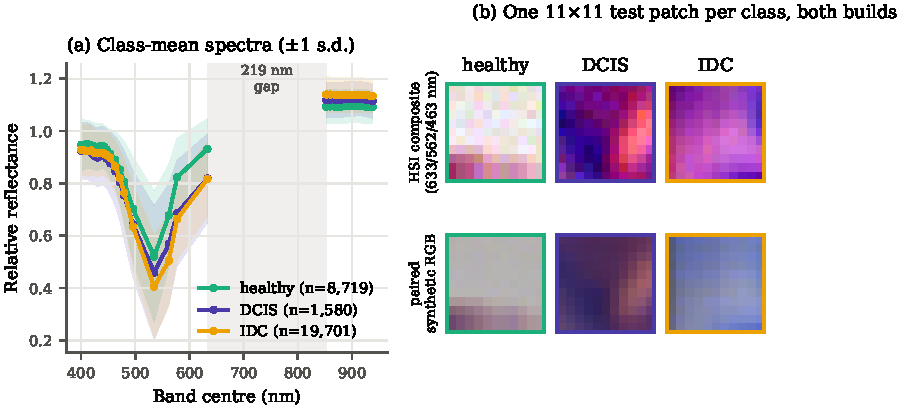
\includegraphics[width=\linewidth]{fig_dataset}
\caption{(a) Class-mean reflectance over the 32 selected bands, 30,000 training patches. (b) One test patch per class as HSI composite (633/562/463~nm) and paired synthetic RGB}
\label{fig:dataset}
\end{figure}

\subsection{Paired Hyperspectral and RGB Builds}\label{sec:paired}
Two builds are written from the same captures, paired at the patch level: the RGB patch is sampled at the \emph{same coordinates} as the cube, with identical patient and capture identifiers. We use the synthetic RGB rendering computed from each cube by the collection's software~\cite{hsibc_desc}, aligned with it in all 644 captures. The arms still differ in more than channel count: the RGB arm is an 8-bit rendering of the full cube and the HSI arm floating-point reflectance at 32 label-selected bands; the reconstruction target has 3 or 32 channels; and the 3-band arm, which carries no band centres, uses the index encoding of Sect.~\ref{sec:pathway}.

\subsection{PAD-UFES-20}
PAD-UFES-20~\cite{pad_desc,pad_data} contains 2,298 smartphone photographs of skin lesions from 1,373 patients in six classes, with melanoma at 2.3\,\%. It is one of MedMamba's datasets; we use a patient-disjoint 70/15/15 split (1,626 / 328 / 344 images), whereas the published MedMamba results use an image-level split.

%======================================================================
\section{Methodology}
%======================================================================
An input patch is $X \in \mathbb{R}^{C \times H \times W}$ with $C$ bands, optionally with band centres $\lambda \in \mathbb{R}^{C}$ in nanometres. Both proposed models share the spectral pathway of Sect.~\ref{sec:pathway}, which maps $X$ to a context map $c \in \mathbb{R}^{H_p \times W_p \times d_{\text{ctx}}}$ whose shape contains no reference to $C$. Appendix~A.1 lists every change component by component and traces the tensor shapes.

\subsection{Base Architectures}
\subsubsection{MedMamba.}
MedMamba~\cite{medmamba} embeds the input with a strided convolution of kernel and stride $p$ and layer normalization,
\begin{equation}
E = \mathrm{LN}\big(W_e \ast_p X + b_e\big), \qquad W_e \in \mathbb{R}^{D_0 \times C \times p \times p},
\label{eq:embed}
\end{equation}
which holds $p^2 C D_0 + 3 D_0$ parameters, linear in $C$ (4,896 at $C=3$ and 49,440 at $C=32$ for $p=4$, $D_0=96$). Four stages follow, separated by patch merging (MedMamba-T: widths 96--768, depths 2, 2, 4, 2). An SS-Conv-SSM block splits the channels into halves $[x_L, x_R]$ and computes
\begin{equation}
x \leftarrow \mathrm{Shuffle}_2\big([\Phi(x_L) \,;\, \mathrm{DropPath}(\mathrm{SS2D}(\mathrm{LN}(x_R)))]\big) + x,
\label{eq:ssconv}
\end{equation}
where $\Phi$ is a convolutional branch with batch normalization, SS2D sums four directional scans~\cite{vmamba}, and $\mathrm{Shuffle}_2$ interleaves the two groups; the classifier reads the last stage. Its one component that cannot serve a variable number of bands is~(\ref{eq:embed}).

\subsubsection{Tiny Recursive Model.}
TRM~\cite{trm} applies one two-layer network $f$ (a token mixer and SwiGLU~\cite{glu}, each followed by RMS normalization~\cite{rmsnorm}) to a latent state $z$ and an answer state $y$, given an embedded input $x$:
\begin{equation}
z \leftarrow f(x, y, z) \;\; (n \text{ times}), \qquad y \leftarrow f(y, z).
\label{eq:trm}
\end{equation}
A recursion runs $T$ such steps, the first $T{-}1$ without gradient; deep supervision runs up to 16 recursions, each with its own loss and optimizer update on detached states, with a halting head and an exponential moving average (EMA) of the weights.

\subsection{The Band-Count-Agnostic Spectral Pathway}\label{sec:pathway}
Every operation shares its weights across the band axis or has none. \emph{Patchification} is parameter-free average pooling, $\bar{X} = \mathrm{AvgPool}_p(X)$; $v \in \mathbb{R}^C$ denotes the spectrum at one position. \emph{Spectral position}: band centres are normalized by the extent of the bands present, and a sinusoidal basis is evaluated on the result,
\begin{align}
\tilde{\lambda}_c &= \frac{\lambda_c - \min_{c'} \lambda_{c'}}{\max_{c'} \lambda_{c'} - \min_{c'} \lambda_{c'}}, \nonumber\\
\pi_c[2i] &= \sin(\eta \tilde{\lambda}_c \omega_i),\quad \pi_c[2i{+}1] = \cos(\eta \tilde{\lambda}_c \omega_i),\quad \omega_i = 10000^{-2i/d_t},\quad \eta = C.
\label{eq:pos}
\end{align}
Without band centres, $\tilde{\lambda}_c = c/(C-1)$, an index encoding, which the wavelength encoding equals for evenly spaced bands. Since the normalization and $\eta$ depend on the bands present, a wavelength's code changes when bands are removed (Sect.~\ref{sec:bands}). \emph{Tokenization}: one two-layer MLP, shared by all bands, lifts each band value with its encoding to a token of width $d_t$,
\begin{equation}
t_c = W_2\, \mathrm{GELU}\big(W_1 [v_c \,;\, \pi_c] + b_1\big) + b_2 + g_s \pi_c;
\label{eq:tok}
\end{equation}
a linear map $v_c \mapsto v_c w$ would also be shape-independent, but would place all band values along one direction. \emph{Spectral encoding}: tokens $\mathcal{T} \in \mathbb{R}^{C \times d_t}$ pass through residual convolution blocks along the band axis and, after the first block, a bidirectional selective scan~\cite{mamba}:
\begin{align}
\mathcal{T} &\leftarrow \mathcal{T} + W_r\, \mathrm{GELU}\big(\mathrm{Conv1d}_3(\mathrm{LN}(\mathcal{T}))\big), \label{eq:conv1d}\\
\mathcal{T} &\leftarrow \mathcal{T} + \Big(\mathrm{LN}\big(\alpha_1 \mathrm{SSM}(U) + \alpha_2 \mathrm{Flip}(\mathrm{SSM}(\mathrm{Flip}(U)))\big) \odot \mathrm{SiLU}(Z)\Big) W_{\text{out}}, \label{eq:scan}
\end{align}
with $[U;Z] = \mathrm{LN}(\mathcal{T})W_{\text{in}}$ and $\alpha = \mathrm{softmax}(a)$. The scan~(\ref{eq:scan}) has the gated form of SS2D, applied to the one axis MedMamba does not model. \emph{Gating and pooling}: a gate weights each band, the tokens are averaged over bands and compressed by three linear layers with GELU ($d_t \to 128 \to 64 \to d_{\text{ctx}}$):
\begin{equation}
a_c = \sigma\big(w_g^{\top} t_c + b_g\big), \quad t_c \leftarrow a_c t_c, \qquad c_{ij} = \Psi\Big(\tfrac{1}{C}\textstyle\sum_{c} t_c\Big) \in \mathbb{R}^{d_{\text{ctx}}}.
\label{eq:pool}
\end{equation}
The mean is where the band axis disappears. We use $d_t = 32$ and $d_{\text{ctx}} = 64$.

\begin{proposition}\label{prop:agnostic}
Every parameter tensor in (\ref{eq:pos})--(\ref{eq:pool}) has a shape determined by $d_t$, $d_{\text{ctx}}$, the kernel width, the scan state size and the compressor widths, not by $C$, and every module after (\ref{eq:pool}) receives inputs without $C$ in their shape. A model built on the pathway whose later modules also produce outputs without $C$ in their shape therefore has the same parameter count at every band count.
\end{proposition}
\begin{proof}
(\ref{eq:pos}) has no parameters. The MLP of (\ref{eq:tok}) is applied per band with shared weights of shapes $2d_t \times (1 + d_t)$ and $d_t \times 2d_t$. The kernel of (\ref{eq:conv1d}) has shape $d_t \times d_t \times 3$ and slides along the bands; the scan (\ref{eq:scan}) shares its parameters along the sequence; the gate is a $1 \times d_t$ projection applied to every band; the mean has no parameters. A module with one output channel per band, such as the optional reconstruction decoder, falls outside the statement. \qed
\end{proof}

The pathway holds 38,724 parameters (tokenizer 4,257; spectral encoder with three blocks and one scan 17,794; gate 33; compressor 16,640), with no term in $C$.

\subsection{MedMamba-SS}\label{sec:ss}
MedMamba-SS keeps the MedMamba hierarchy, replaces (\ref{eq:embed}), the only layer whose weights depend on $C$, and lets the spectrum inform every scale. \emph{Stem}: the first stage receives $F^{(1)} = \mathrm{LN}(W_s\, \rho(c) + b_s)$, where $\rho(c) = c/\mathrm{RMS}(c)$ is a parameter-free RMS normalization with no $\epsilon$ added to the mean square, which keeps the stem responsive when the context is small in magnitude (Appendix~A.2). \emph{Per-stage conditioning}: at stage $s$ the resized context is re-weighted by a squeeze-and-excitation gate~\cite{senet} and modulates every block through FiLM~\cite{film}, initialized to the identity:
\begin{equation}
\begin{split}
c_s &\leftarrow c_s \odot \sigma\big(W_{b,2}\,\mathrm{GELU}(W_{b,1}\,\mathrm{GAP}(c_s))\big), \\
\tilde{x} &= x \odot (1 + \gamma) + \beta, \qquad [\gamma ; \beta] = W_f c_s + b_f,
\end{split}
\label{eq:film}
\end{equation}
\emph{Conditioned block}: MedMamba's split, convolutional branch, shuffle and outer residual are kept; the scan half is added back to its scan output, both residual branches are scaled by LayerScale~\cite{layerscale} (LS, initialized at $10^{-4}$), SS2D combines its four scans with learned softmax weights, and a GEGLU feed-forward sublayer $G$~\cite{glu} is appended:
\begin{equation}
\begin{split}
x &\leftarrow \mathrm{Shuffle}_2\big([\Phi(\tilde{x}_L) \,;\, \tilde{x}_R + \mathrm{LS}(\mathrm{SS2D}(\mathrm{LN}(\tilde{x}_R)))]\big) + x,\\
x &\leftarrow x + \mathrm{LS}(G(\mathrm{LN}(x))).
\end{split}
\label{eq:block}
\end{equation}
\emph{Context update and head}: after a stage's blocks, $c_s \leftarrow \mathrm{LN}(c_s + \sigma(W_g c_s) \odot W_u F^{(s)})$ feeds spatial features back to the context, and the classifier is an MLP on the pooled features of every stage and $\mathrm{GAP}(c_S)$. \emph{Configurations}: for 11$\times$11 hyperspectral patches, $p=1$ and three stages of widths 64, 128, 256 with two blocks each (2,773,007 parameters); for 224$\times$224 photographs, MedMamba-T's layout with $p=8$ (27,425,314 parameters). A \emph{full-channel} variant removes the channel split, both branches seeing all channels and combined by learned gating (3,513,451 parameters on 11$\times$11 patches).

\subsection{MedMamba-SS-TRM}\label{sec:sstrm}
MedMamba-SS-TRM keeps the spectral pathway and the task interface of MedMamba-SS and replaces the hierarchy by one core of width $d = 128$ applied many times. \emph{Stem and states}: $x = \mathrm{LN}(W_s\, \rho(c) + b_s) + g_p P$, with $P$ a fixed 2-D sinusoidal encoding and $g_p$ a learnable gain; $x$ is held fixed, and $y$, $z$ start from non-trainable buffers as in TRM. \emph{Core}: $f = B_2 \circ B_1$, each block a token mixer and a GEGLU MLP under parameter-free RMS post-normalization~\cite{rmsnorm}:
\begin{equation}
h' = \mathrm{RMS}(h + M(h)), \;\; B(h) = \mathrm{RMS}(h' + G(h')), \;\; M(h) = G_m(\mathrm{DWConv}_{3\times3}(h)).
\label{eq:core}
\end{equation}
The depthwise 3$\times$3 convolution with a channel MLP replaces TRM's sequence mixer because the state is a 2-D grid; SS2D and self-attention are implemented alternatives. \emph{Recursion, head and objective}: the improvement step instantiates (\ref{eq:trm}) with additive input injection, the classifier reads the answer state after every segment $j$, and the per-segment losses are averaged:
\begin{equation}
z \leftarrow f(z + y + x)\ (n \text{ times}), \;\; y \leftarrow f(y + z), \qquad \ell_j = W_c\, \mathrm{GAP}(\mathrm{LN}(y^{(j)})) + b_c,
\label{eq:recursion}
\end{equation}
\begin{equation}
\mathcal{L} = \frac{1}{N_{\text{sup}}} \sum_{j=1}^{N_{\text{sup}}} \mathcal{L}_{\text{FL}}(\ell_j, k) + \lambda_{\text{mse}}\, \mathrm{MSE}(\hat{X}, X) + \lambda_{\text{sam}}\, \mathrm{SAM}(\hat{X}, X),
\label{eq:loss}
\end{equation}
where $\mathcal{L}_{\text{FL}}$ is the focal loss (\ref{eq:focal}), $\hat{X}$ the output of a three-layer convolutional decoder reading the final answer state, SAM the per-pixel spectral angle between $\hat{X}$ and $X$, and $\lambda_{\text{mse}} = \lambda_{\text{sam}} = 0.1$. All $N_{\text{sup}} = 3$ segments run inside one forward pass with one optimizer update per batch (Algorithm~\ref{alg:forward}, Appendix~A.1), so with $n = 6$ and $T = 3$ the core is applied $K = N_{\text{sup}} T (n+1) = 63$ times per forward pass, at inference as in training. Evaluation uses an EMA of the weights (decay 0.9995), and every gradient-carrying core call is checkpointed~\cite{checkpointing}. The model has 446,409 parameters, 89.2\,\% of them in the core (Table~\ref{tab:params}), and none depends on $K$ or $C$.

\emph{Lineage.} TRM's two-state recursion, input injection, gradient-free prelude and detach between segments are used as specified~\cite{trm}; deep supervision moves inside one forward pass, and halting is disabled because the halting head does not learn here (Appendix~A.2). The spatial mixer is convolutional because an SS2D mixer without a fused kernel was 39 times slower (Sect.~\ref{sec:setup}), so no SS-Conv-SSM block remains; the name records the lineage through MedMamba-SS, whose spectral pathway and selective scan are kept, not a spatial state-space backbone.

\subsection{Cost Model}\label{sec:cost}
Weight sharing decouples parameters from arithmetic: the core's parameters, $L(12d^2 + 20d)$, do not depend on $K$, but its arithmetic grows linearly,
\begin{equation}
\mathcal{F}(K) = \mathcal{F}_0 + K \mathcal{F}_f, \qquad \mathcal{F}_f = 2 N_{\text{tok}} L \big(12 d^2 + 9 d\big),
\label{eq:cost}
\end{equation}
where $12d^2$ counts the multiply--accumulates per token of a block's two GEGLU MLPs, $9d$ the depthwise convolution, and $N_{\text{tok}} = H_p W_p$. For 11$\times$11 patches, $L = 2$ and $d = 128$, $\mathcal{F}_f = 95.72$~MFLOPs, so the 63 applications cost 6.03~GFLOPs. Measured arithmetic counts the multiply--accumulates of every convolution and linear layer with forward hooks, doubled, plus an analytic estimate for the scans, without the reconstruction decoder; it says nothing about latency. MedMamba-SS costs 0.278~GFLOPs on the same input: a hierarchy reduces its token count at every stage, whereas every core application pays for the full 121-token grid.

%======================================================================
\section{Experimental Setup}\label{sec:setup}
%======================================================================
\subsubsection{Loss and Metrics.}
Classification uses the focal loss~\cite{focal} with class weights against the 13\,:\,1 class imbalance. For a patch of class $k$ with predicted probability $p_k$ and $N_k$ training patches per class,
\begin{equation}
\mathcal{L}_{\text{FL}} = -\,w_k\,(1 - p_k)^{\gamma} \log p_k, \quad \gamma = 1.5, \qquad
w_k \propto \Big(\frac{N}{K_{\text{cls}} N_k}\Big)^{0.75},
\label{eq:focal}
\end{equation}
The weights are normalized to sum to $K_{\text{cls}}$. Balanced accuracy (BA, the mean per-class recall) and macro-F1 are the primary metrics. Calibration is measured by the expected calibration error (ECE) over 15 bins~\cite{naeini,guo2017} and the Brier score~\cite{brier}; reconstruction by the spectral angle on reflectance with RMSE, PSNR and 2-D SSIM; and per-patient macro recall is the mean recall over the classes a patient has.

\subsubsection{Implementation.}
All models were trained on one NVIDIA RTX 5060 Ti (16~GB) with PyTorch 2.11~\cite{pytorch}. MedMamba-SS-TRM uses AdamW~\cite{adamw} at learning rate $3 \times 10^{-4}$ with weight decay 0.05, batch size 256, bf16, gradient clipping at 1.0, and a 587-step warmup into cosine decay over 19,560 steps (Table~\ref{tab:config}). Each epoch trains on a fresh random 10.2\,\% of the training split (250,113 patches) and validates on a fixed patient-stratified 9.86\,\% of the validation split (32,985 patches); the checkpoint with the best validation macro-F1 is tested on the full test split. Headline runs train for 20 epochs, ablations for 12 epochs against a 12-epoch baseline. The recipe was developed over earlier runs on the same split: checkpoints were always selected on validation data, but test scores of development runs were recorded, so the test patients are independent of checkpoint selection but not demonstrably of recipe development. In a benchmark on RGB skin-lesion patches, replacing only the SS2D mixer (66.9~s per step, no fused kernel) by the convolutional one made the step 39 times faster. Every run passes validity gates (leakage, representation-sensitivity, split-drift and reconstruction-gradient checks).

\subsubsection{Baselines.}
All baselines use the same HSI build and patient split. (i)~\emph{Shallow probes}: class-balanced logistic regressions~\cite{sklearn} on per-band means (32 features), means and standard deviations (64), and the flattened patch (3,872), fitted on 25,000 training patches. (ii)~\emph{MedMamba}~\cite{medmamba}: the reference implementation with a 32-band stem, patch size 1, widths (64, 128, 256, 512) and depths (1, 1, 2, 1), 3,648,995 parameters, trained for five full epochs with class-weighted cross-entropy under its own recipe; its checkpoint (epoch 1) was chosen on the full validation split, the set on which its validation scores are reported. (iii)~\emph{HybridSN}~\cite{hybridsn} (569,843 parameters, applied without padding to the 32 bands of the 11$\times$11 patch) and \emph{SpectralFormer}~\cite{spectralformer} (121,428 parameters, patch-wise variant with official defaults), trained with MedMamba-SS-TRM's 20-epoch recipe without EMA or reconstruction and not tuned; neither is band-count agnostic. (iv)~\emph{MedMamba-SS} under MedMamba-SS-TRM's recipe at the 12-epoch budget.

\subsubsection{Protocol.}
The HSI-versus-RGB comparison repeats both arms at five seeds (1, 7, 13, 23, 42); HybridSN and SpectralFormer are trained at the same seeds, and every other configuration uses seed~42. Two pairs of identical runs differ by 0.04 and 0.06 points of BA, whereas changing the seed moves test BA by s.d.\ 1.9 points. Every selected checkpoint is also evaluated on the \emph{full} validation split, so that all ten non-training patients can be analysed; because the validation patients also select each network's checkpoint, validation and pooled scores of the networks are optimistic (the probes involve no selection). Patient-level 95\,\% intervals resample held-out patients (2,000 draws) and discard draws that lose a class, so they condition on the DCIS patient being present.

%======================================================================
\section{Results}
%======================================================================
\subsection{Comparison with Existing Models}\label{sec:comparison}

\begin{table}[t]
\caption{Comparison on HistologyHSI-BC-Recurrence (seed 42 unless stated; ``5 s.'': mean\,\pt\,s.d.\ over seeds 1, 7, 13, 23, 42). BA: balanced accuracy (\%); F1: macro-F1; Pool.: all 10 held-out patients; LR: logistic regression}
\label{tab:main}
\centering\scriptsize
\setlength{\tabcolsep}{1.5pt}
\begin{tabular}{@{}lrrrrrr@{}}
\toprule
Model & Params & Test BA & Test F1 & Val.\ BA & Pool.\ BA & Pool.\ F1 \\
\midrule
Majority class (IDC) & --- & 33.33 & 0.272 & 33.33 & 33.33 & 0.266 \\
LR, band means & 32 f. & 82.68 & 0.726 & 68.39 & 75.81 & 0.671 \\
LR, band means + s.d. & 64 f. & 90.28 & 0.843 & 77.99 & 84.31 & 0.771 \\
LR, raw patch & 3,872 f. & 62.02 & 0.623 & 56.92 & 59.86 & 0.587 \\
LR, RGB means + s.d.\ (RGB) & 6 f. & 87.58 & 0.830 & 84.90 & 86.50 & 0.807 \\
MedMamba~\cite{medmamba} & 3.649\,M & 91.02 & 0.872 & 72.30 & 81.67 & 0.774 \\
HybridSN~\cite{hybridsn} & 0.570\,M & 88.85 & 0.841 & 84.94 & 87.14 & 0.813 \\
HybridSN, 5 s. & 0.570\,M & 89.40\sd{0.47} & 0.841\sd{0.008} & 84.37\sd{1.04} & 87.12\sd{0.66} & 0.813\sd{0.013} \\
SpectralFormer~\cite{spectralformer} & 0.121\,M & 82.45 & 0.804 & 80.73 & 81.78 & 0.784 \\
SpectralFormer, 5 s. & 0.121\,M & 83.02\sd{3.98} & 0.817\sd{0.025} & 79.29\sd{1.29} & 81.30\sd{2.33} & 0.788\sd{0.013} \\
MedMamba-SS (12 ep.) & 2.773\,M & 33.42 & 0.274 & 33.30 & 33.36 & 0.267 \\
MedMamba-SS, full-ch.\ (12 ep.) & 3.513\,M & 40.85 & 0.397 & 30.20 & 35.64 & 0.329 \\
\textbf{MedMamba-SS-TRM} & \textbf{0.446\,M} & 94.37 & 0.904 & 72.11 & 83.21 & 0.795 \\
\textbf{MedMamba-SS-TRM}, 5 s. & 0.446\,M & 92.78\sd{1.87} & 0.875\sd{0.040} & 76.18\sd{4.59} & 84.49\sd{1.45} & 0.795\sd{0.012} \\
\bottomrule
\end{tabular}
\end{table}

On the test patients MedMamba-SS-TRM has the highest BA (92.78\ms1.87\,\% over five seeds, 94.37\,\% at seed 42), ahead of MedMamba (91.02\,\%), the 64-feature probe (90.28\,\%), HybridSN and SpectralFormer (Table~\ref{tab:main}); at seed~1 (89.61\,\%) MedMamba and the 64-feature probe are ahead. On the other test metrics the five-seed mean does not lead MedMamba: macro-F1 is level (0.875 against 0.872), and accuracy (94.66 against 95.14\,\%) and Cohen's $\kappa$ (0.888 against 0.896) are lower. On the validation patients the order reverses: HybridSN (84.94\,\%) and a six-feature RGB colour probe (84.90\,\%) lead, and MedMamba-SS-TRM (76.18\ms4.59\,\%) and MedMamba (72.30\,\%) trail the 64-feature probe. Seed 42 is MedMamba-SS-TRM's best test seed and worst validation seed (across seeds, Pearson $r = -0.95$ between the two).

\emph{Seed-paired baselines.} On the test patients MedMamba-SS-TRM is ahead of SpectralFormer at every seed, by 9.77\ms4.25 points of BA, and of HybridSN at four of five seeds, by 3.38\ms2.14 points (level at seed~1: 89.61 against 89.65\,\%). On the validation patients HybridSN is ahead at every seed, by 8.19\ms4.44 points, and SpectralFormer at four of five, by 3.11\ms5.64. Pooled over all ten held-out patients, HybridSN is ahead of MedMamba-SS-TRM at every seed, by 2.62\ms1.34 points (87.12\ms0.66 against 84.49\ms1.45\,\%), and MedMamba-SS-TRM is ahead of SpectralFormer at four of five, by 3.19\ms2.94. The ranking thus depends on which five patients are held out more than on the architecture: among the networks that train, the test--validation gap ranges from 1.7 points (SpectralFormer) to 22.3 points (MedMamba-SS-TRM at seed 42). Linear models on 64 band statistics or six colour statistics are competitive with every network.

\subsection{Band-Count Agnosticism}\label{sec:bands}
\emph{Structure.} The same MedMamba-SS-TRM has exactly 446,409 parameters at 32 and at 3 bands, as Proposition~\ref{prop:agnostic} predicts (parameter memory 1.786~MB in both cases). Activation size (peak inference memory 161.5 against 52.6~MB) and, marginally, arithmetic (6.203 against 6.052~GFLOPs) depend on the band count; the reconstruction decoder, whose output has one channel per band, is excluded from all counts.

\emph{Behaviour.} Fig.~\ref{fig:bands} evaluates the seed-42 model on index-decimated subsets of its bands without retraining (\emph{zero-shot}) and trains fresh models at 16 and 8 bands (\emph{retrained}, 12 epochs). With the encoding as defined, zero-shot transfer fails: BA falls to 0.33--0.41 and IDC F1 to 0.000 at every reduced band count. At 16 bands this failure comes from the encoding: decimation keeps both end bands, so the normalization in (\ref{eq:pos}) is unchanged, but $\eta = C$ changes, giving every retained band a code unseen in training. Holding $\eta$ at its training value of 32, and nothing else, raises BA from 0.3845 to 0.9086 and macro-F1 from 0.1854 to 0.8256 at 16 bands; at 8 bands BA rises only from 0.3329 to 0.5599. With all 32 bands the fixed encoding reproduces the model's own result (macro-F1 0.90365 against 0.90363). These are single post-hoc evaluations of one checkpoint. Retrained at eight bands, the model reaches 0.9014 BA and 0.8684 macro-F1, 96 and 97\,\% of the 12-epoch 32-band values (0.9353 and 0.8920); the 3.4-point loss is about 1.3 times the s.d.\ expected between two single runs. The bands were decimated from a label-selected set of narrow bands, so the result does not carry over directly to a filter camera with broader bands.

\begin{figure}[t]
\centering
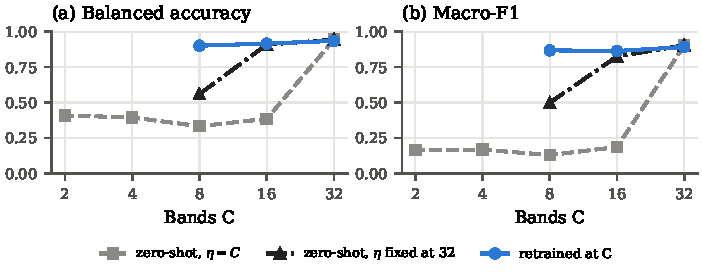
\includegraphics[width=0.92\linewidth]{fig_bands}
\caption{Test performance against band count: zero-shot with $\eta = C$ or $\eta$ fixed at 32 (seed-42 model), and retrained at $C$ (12 epochs)}
\label{fig:bands}
\end{figure}

\subsection{Ablations and the Hierarchical Backbone}\label{sec:ablation}
Table~\ref{tab:ablation} removes one component at a time at the 12-epoch budget; the last two rows put the hierarchical MedMamba-SS backbone back in place of the recursive core. Removing the reconstruction objective lowers BA by 1.3 points and macro-F1 by 0.021, mostly in DCIS, and replacing the wavelength encoding with an index encoding lowers them by 0.6 points and 0.012; both effects are smaller than the seed-to-seed s.d.\ (1.9 points), so they are consistent with a contribution but do not establish one.

\begin{table}[t]
\caption{Component ablations (test, 12-epoch budget, seed 42)}
\label{tab:ablation}
\centering\scriptsize
\setlength{\tabcolsep}{4pt}
\begin{tabular}{@{}lrrrr@{}}
\toprule
Variant & BA & Macro-F1 & DCIS F1 & $\Delta$ macro-F1 \\
\midrule
MedMamba-SS-TRM, full & \textbf{0.9353} & \textbf{0.8920} & \textbf{0.769} & --- \\
$-$ reconstruction objective ($\lambda = 0$) & 0.9225 & 0.8708 & 0.733 & $-$0.021 \\
$-$ wavelength encoding (index encoding), run 1 & 0.9291 & 0.8804 & 0.748 & $-$0.012 \\
$-$ wavelength encoding (index encoding), run 2 & 0.9287 & 0.8798 & 0.747 & $-$0.012 \\
16 bands (retrained) & 0.9159 & 0.8636 & 0.717 & $-$0.028 \\
8 bands (retrained) & 0.9014 & 0.8684 & 0.715 & $-$0.024 \\
21 core applications instead of 63 & 0.9378 & 0.8932 & 0.774 & +0.001 \\
hierarchical backbone (MedMamba-SS) & 0.3342 & 0.2741 & 0.001 & $-$0.618 \\
hierarchical backbone, full-channel & 0.4085 & 0.3974 & 0.228 & $-$0.495 \\
\bottomrule
\end{tabular}
\end{table}

The hierarchical MedMamba-SS stays at chance under the recursive model's recipe: both variants select their first epoch, and lower learning rates, removing the decoder or a higher clipping threshold leave it there. Its training accuracy rises (0.735 to 0.906) while validation macro-F1 stays at 0.2583, that of a constant prediction, pointing to a module that behaves differently in evaluation mode: $\Phi$ contains batch normalization. With test-batch statistics the prediction no longer collapses, but BA reaches only 0.490 on a stratified test sample (Appendix~A.3), for reasons not identified. On hyperspectral patches the recursive substitution is therefore established on parameters, arithmetic and interface, and its quality is compared against MedMamba rather than MedMamba-SS.

\subsection{Recursion Depth and Computational Cost}\label{sec:depth}
Varying only the number of improvement steps ($T = 1$ to 4; Fig.~\ref{fig:depth}), quality is flat and non-monotonic (BA 0.9378, 0.9441, 0.9353 and 0.9386 at 21, 42, 63 and 84 core applications), within noise at one seed. Measured arithmetic is 2.183, 4.193, 6.203 and 8.213~GFLOPs, a straight line with the slope of (\ref{eq:cost}), 95.72~MFLOPs per application, on an intercept of 0.173~GFLOPs. On the same input MedMamba-SS-TRM holds 6.2 times fewer parameters than MedMamba-SS (446,409 against 2,773,007) and needs 22.3 times more arithmetic (6.203 against 0.278~GFLOPs); on 224$\times$224 RGB images the ratios are 61.4 and 16.4. Because the forward pass always runs all segments, inference pays this cost too: parameter count in a weight-shared recursive model measures storage, not compute.

\begin{figure}[t]
\centering
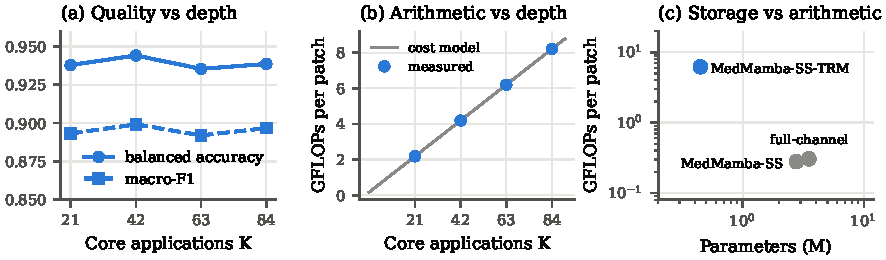
\includegraphics[width=0.92\linewidth]{fig_recursion_cost}
\caption{(a) Test quality against core applications (12 epochs). (b) Measured arithmetic against the cost model~(\ref{eq:cost}). (c) Parameters against arithmetic}
\label{fig:depth}
\end{figure}

\subsection{Hyperspectral Versus RGB Input}\label{sec:modality}
The same model is trained on the paired RGB build, sharing recipe, split and patch coordinates (Table~\ref{tab:modality}).

\begin{table}[t]
\caption{BA (\%) of the 32-band (HSI) and 3-band (RGB) arms of MedMamba-SS-TRM; $\Delta$ in points}
\label{tab:modality}
\centering\scriptsize
\setlength{\tabcolsep}{4pt}
\begin{tabular}{@{}lrrrrrrrrr@{}}
\toprule
& \multicolumn{3}{c}{Test (5 patients)} & \multicolumn{3}{c}{Validation (5 patients)} & \multicolumn{3}{c}{Pooled (10 patients)} \\
\cmidrule(lr){2-4}\cmidrule(lr){5-7}\cmidrule(l){8-10}
Seed & HSI & RGB & $\Delta$ & HSI & RGB & $\Delta$ & HSI & RGB & $\Delta$ \\
\midrule
1 & 89.61 & 88.18 & +1.43 & 83.00 & 84.81 & $-$1.81 & 86.32 & 86.73 & $-$0.41 \\
7 & 93.41 & 88.97 & +4.45 & 74.37 & 80.41 & $-$6.05 & 83.94 & 84.89 & $-$0.95 \\
13 & 92.76 & 88.79 & +3.97 & 78.66 & 78.94 & $-$0.28 & 85.74 & 83.99 & +1.75 \\
23 & 93.78 & 88.89 & +4.88 & 72.77 & 82.39 & $-$9.62 & 83.26 & 85.86 & $-$2.59 \\
42 & 94.37 & 88.51 & +5.86 & 72.11 & 83.41 & $-$11.31 & 83.21 & 86.17 & $-$2.96 \\
\textbf{Mean} & \textbf{92.78} & \textbf{88.67} & \textbf{+4.12} & \textbf{76.18} & \textbf{81.99} & \textbf{$-$5.81} & \textbf{84.49} & \textbf{85.53} & \textbf{$-$1.04} \\
s.d.\ of $\Delta$ & & & 1.66 & & & 4.78 & & & 1.89 \\
\bottomrule
\end{tabular}
\end{table}

On the test patients BA favours 32-band input at five of five seeds, by 4.12\ms1.66 points, with the gain in healthy tissue and DCIS (mean per-class F1 0.892 against 0.844 and 0.739 against 0.656; IDC 0.993 against 0.994). On the validation patients the sign reverses: 3-band input is better at five of five seeds, by 5.81\ms4.78 points; pooled, the difference is $-$1.04\ms1.89. Resampling patients, the 95\,\% interval of the seed-mean difference is [+1.6,\,+4.8] points on test, [$-$11.8,\,$-$1.4] on validation and [$-$6.6,\,+3.9] pooled. Averaged over seeds (Fig.~\ref{fig:modality}(b)), 32-band input gives the higher macro recall for seven of the ten held-out patients; patient 136 is tied at 0.770, patient 197 narrowly favours 3 bands (0.853 against 0.866), and patient 304 favours them widely (0.566 against 0.773). Without patient 304 the validation difference shrinks to $-$1.91\ms5.50 points. The same patient reverses the comparison without any network: the 64-feature probe scores 90.28 with 32 bands against 87.58\,\% with 3 on test, and 77.99 against 84.90\,\% on validation, where patient 304 again favours 3 bands (0.672 against 0.836). The comparison therefore does not establish that 32-band input is better: ten patients, with one DCIS patient per held-out set, are too few to decide, and the label-informed band selection could favour the 32-band arm.

\begin{figure}[t]
\centering
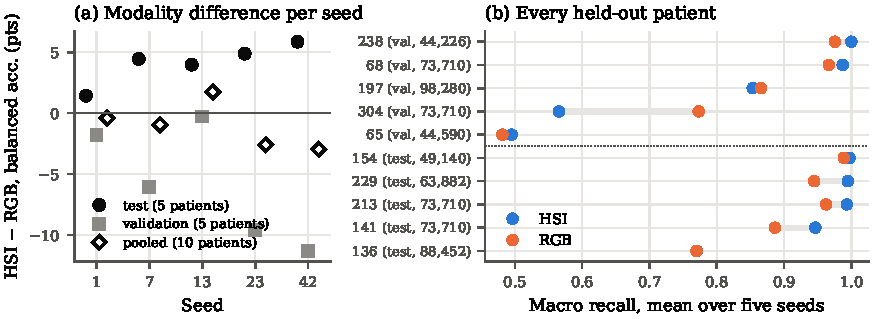
\includegraphics[width=0.92\linewidth]{fig_modality}
\caption{(a) HSI $-$ RGB balanced accuracy per seed. (b) Macro recall of every held-out patient (split, number of patches), mean over five seeds}
\label{fig:modality}
\end{figure}

\subsection{Errors and Calibration}\label{sec:errors}
Both arms classify IDC almost perfectly, so the healthy-tissue errors are DCIS predictions (14.3\,\% of healthy patches with 32 bands and 27.5\,\% with 3 at seed 42). The errors are concentrated in individual patients at every seed and in both arms (Table~\ref{tab:perpatient}): test patient 136, the only test patient with DCIS, produces 83\,\% of the seed-42 healthy errors, validation patient 304 has healthy recall 0.01--0.30 with 32 bands against 0.50--0.62 with 3, and the ten small IDC captures of patient 65 are almost never classified as IDC. On the test patients the 32-band model is better calibrated than its 3-band twin (ECE 0.056\ms0.007 against 0.094\ms0.017) but under-confident, whereas every model with validation predictions is over-confident on the validation patients, so a temperature~\cite{guo2017} fitted on one set does not transfer to the other (Appendix~A.3).

\subsection{Band Gate and Reconstruction}\label{sec:xai}
Averaged over 9,000 class-stratified test patches, the band gate (\ref{eq:pool}) rises from about 0.55 below 500~nm to a peak at 577~nm, stays high to 633~nm and falls to about 0.54 in the near-infrared, highest for DCIS (0.67), where the class spectra differ most (Fig.~\ref{fig:xai}, Appendix~A.3). It is a learned weighting, not a causal attribution, and every DCIS test patch comes from one patient.

The auxiliary decoder reconstructs the 32-band input from the final answer state (Fig.~\ref{fig:recon}). On the validation subset its spectral angle falls from 9.47$^\circ$ after the first epoch to 6.16$^\circ$ at the selected epoch 7 (RMSE 0.1109; PSNR 20.3~dB as a batch-weighted mean of per-batch values). Median reconstructions follow the input spectrum across both spectral regions, including the absorption minimum near 535~nm, and preserve the spatial pattern (2-D SSIM 0.66--0.80). The worst IDC patch (20.6$^\circ$) is saturated and lacks the stain absorption minimum.

\begin{figure}[t]
\centering
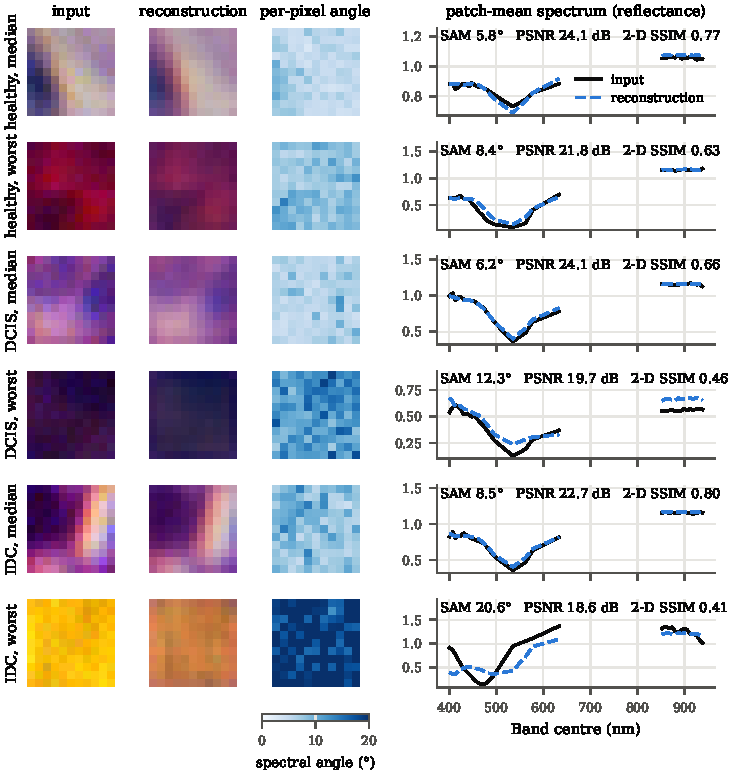
\includegraphics[width=0.72\linewidth]{fig_reconstruction}
\caption{Reconstruction on validation patches: median and worst patch per class by spectral angle; composites 633/562/463~nm}
\label{fig:recon}
\end{figure}

\subsection{Skin Lesions}\label{sec:pad}
On PAD-UFES-20, 11$\times$11 patches inherit the photograph's label although most contain no lesion, a multiple-instance setting~\cite{ilse}: MedMamba-SS-TRM reaches only 25.7\,\% patch-level BA (chance 16.7\,\%), 35.6\,\% when patch predictions are averaged per image. On whole 224$\times$224 images (Table~\ref{tab:pad}, Appendix~A.3) MedMamba-SS trains, well above the majority-class accuracy of 34.6\,\%, so its failure on hyperspectral patches is not a failure of the hierarchy on every input; it has the highest accuracy (53.5\,\%), $\kappa$ and ROC-AUC, and MedMamba-SS-TRM the highest BA (50.2\,\%) and macro-F1 with 61 times fewer parameters. These are confounded single runs (different training sets, recipes and class weighting; a repeat of the MedMamba-SS run moves macro precision by 17 points), so we do not rank the models on them.

%======================================================================
\section{Discussion}
%======================================================================
A trained instance of the pathway transfers only partly: zero-shot at 16 bands it collapses when the encoding scale follows the band count but keeps 0.909 BA when the scale is fixed, which makes a band-count-independent $\eta$, possibly with training on random band subsets~\cite{channelvit}, a candidate design that retraining must confirm. Against MedMamba the recursive model is ahead on test and pooled BA and behind on test accuracy and $\kappa$, but the core also replaces MedMamba's spatial scan, so that comparison measures both changes. Three expectations carried over from TRM do not hold here: the halting head does not learn on three-way tissue labels, 21 core applications match 63, and a weight-shared recursive model is not cheap to run. Whether HSI beats RGB input, and whether MedMamba-SS-TRM beats HybridSN or a linear probe on per-patch statistics, depends on which five patients are held out.

\subsubsection{Limitations.}
\emph{Band selection}: the 32 input bands were chosen with tissue labels from 64 captures drawn before the split, 16 of them from held-out patients; re-selection on training patients moves every band by at most 5.1~nm, but no model has been retrained on that build. \emph{Held-out patients}: all HSI results rest on ten non-training patients with one DCIS patient per held-out set; the validation patients select checkpoints, and test scores of development runs were recorded while the recipe was developed. \emph{Labels}: patches inherit capture labels without a pixel mask, evaluation is per patch rather than per patient, DCIS is the diagnosis on which pathologists agree least often~\cite{elmore}, and the data come from one institution and acquisition system; nothing here constitutes clinical validation. \emph{Statistics}: MedMamba, the probes and every ablation are single runs, HybridSN and SpectralFormer were not tuned, no non-recursive control of the same size was trained, and MedMamba-SS remains unablated on HSI. \emph{Modality}: the RGB input is an 8-bit synthetic rendering, and the arms also differ in reconstruction target and position encoding.

\subsubsection{Future Work.}
Retraining on the training-only band-selection build; patient-level five-fold cross-validation with band selection inside each fold, testing all seven DCIS patients once under a recipe fixed in advance; a second sensor, HMI-LUSC (10 patients, 61 bands from 450 to 750~nm)~\cite{hmilusc}; a non-recursive control and multi-seed ablations; MedMamba-SS with a normalization independent of batch statistics; and a channel-adaptive baseline such as BAT-Former~\cite{batformer}.

%======================================================================
\section{Conclusion}
%======================================================================
We extended MedMamba~\cite{medmamba} in two single substitutions: a spectral pathway whose parameters do not depend on the number of bands (MedMamba-SS), and one weight-shared core applied recursively in the manner of TRM~\cite{trm} (MedMamba-SS-TRM). Two properties follow from the design and are confirmed by measurement, independent of which patients are held out: the classification path has exactly 446,409 parameters at 3 and at 32 bands, and the recursive core reduces parameters 6.2 times while multiplying arithmetic 22.3 times, so parameter count in a weight-shared recursive model measures storage, not compute. The comparisons with other models and with RGB input depend on the patients: MedMamba-SS-TRM has the highest BA on the five test patients (92.8\ms1.9\,\% over five seeds) but HybridSN leads it pooled over all ten at every seed, and the advantage of 32 over 3 bands follows the same split (+4.1 points on test, $-$5.8 on validation, $-$1.0 pooled), as does a linear probe. Whether recursion improves on a non-recursive core of the same size, and whether HSI benefits breast histology classification, remain to be settled on more patients with band selection restricted to training data.

%======================================================================
\section*{Appendix}
%======================================================================
\addcontentsline{toc}{section}{Appendix}
\setcounter{subsection}{0}
\renewcommand{\thesubsection}{A.\arabic{subsection}}

\subsection{Model Details and Component-Level Changes}
Algorithm~\ref{alg:forward} gives the forward pass of MedMamba-SS-TRM and Table~\ref{tab:params} its parameters. Tables~\ref{tab:chg-ss}--\ref{tab:chg-tiny} list every change made by the two substitutions, and Table~\ref{tab:shapes} traces one 11$\times$11 patch through both models.

\begin{algorithm}[H]
\caption{MedMamba-SS-TRM forward pass}\label{alg:forward}
\footnotesize
\begin{algorithmic}[1]
\State $c \gets \mathrm{SpectralPathway}(X, \lambda)$; \ $x \gets \mathrm{Stem}(c)$ \Comment{(\ref{eq:pos})--(\ref{eq:pool}); $x$ held fixed}
\State $y, z \gets y_{\text{init}}, z_{\text{init}}$
\For{$j = 1$ \textbf{to} $N_{\text{sup}} = 3$}
  \State \textbf{repeat} $T-1 = 2$ times without gradient: $(y, z) \gets \mathrm{Improve}(x, y, z)$
  \State $(y, z) \gets \mathrm{Improve}(x, y, z)$ \Comment{carries gradient}
  \State $\ell_j \gets \mathrm{Head}(y)$; \ $y, z \gets \mathrm{detach}(y), \mathrm{detach}(z)$
\EndFor
\State \Return $\ell_1, \ldots, \ell_{N_{\text{sup}}}$ \Comment{inference uses $\ell_{N_{\text{sup}}}$}
\Statex \textbf{Improve}$(x, y, z)$: repeat $n = 6$ times $z \gets f(z + y + x)$; then $y \gets f(y + z)$
\end{algorithmic}
\end{algorithm}

\begin{table}[!htb]
\caption{Parameters of MedMamba-SS-TRM ($d = 128$, $L = 2$ core blocks, three classes)}
\label{tab:params}
\centering\scriptsize
\begin{tabular}{@{}lllrr@{}}
\toprule
Component & Eq. & As a function of width & Count & Share \\
\midrule
Spectral pathway & (\ref{eq:pos})--(\ref{eq:pool}) & Sect.~\ref{sec:pathway} & 38,724 & 8.7\,\% \\
Stem and positional gain & --- & $d_{\text{ctx}} d + 3d + 1$ & 8,577 & 1.9\,\% \\
Shared core & (\ref{eq:core}) & $L(12d^2 + 20d)$ & 398,336 & 89.2\,\% \\
Classifier and halting head & (\ref{eq:recursion}) & $2d + (d+1)(K_{\text{cls}} + 1)$ & 772 & 0.2\,\% \\
\textbf{Total} & & \textbf{no term in $C$} & \textbf{446,409} & \\
\bottomrule
\end{tabular}
\end{table}

\begin{table}[!htb]
\caption{Changes from MedMamba to MedMamba-SS}
\label{tab:chg-ss}
\centering\scriptsize
\setlength{\tabcolsep}{3pt}
\begin{tabular}{@{}L{1.9cm}L{2.4cm}L{3.0cm}L{1.4cm}L{2.55cm}@{}}
\toprule
Component & MedMamba~\cite{medmamba} & MedMamba-SS & Change & Purpose \\
\midrule
Patch embedding & Strided $p\times p$ conv.\ (\ref{eq:embed}); $1{,}536C + 288$ params at $p = 4$ & Average-pool patchify, spectral pathway, linear stem & Replaced & Remove $C$ from every parameter shape; read band order and wavelength \\
Stage input & Previous stage only & Context selector and FiLM (\ref{eq:film}), identity at init. & Added & Condition every scale on the spectrum \\
Split, conv.\ branch, shuffle, outer residual & (\ref{eq:ssconv}) & Same & Unchanged & --- \\
Scan branch & SS2D, four scans summed & Learned direction weights, LayerScale, $x_R$ added back (\ref{eq:block}) & Modified & Residual branch starts near zero; identity path \\
Feed-forward & None & GEGLU with LayerScale (\ref{eq:block}) & Added & Mixing over all channels \\
Context update & None & Gated update from spatial features & Added & Spatial-to-spectral feedback \\
Patch merging & Halve resolution, double width & Same; context pooled alongside & Unchanged & --- \\
Head & GAP of last stage, linear & MLP on all stage pools and spectral summary & Modified & Expose every scale and the spectrum \\
Reconstruction decoder & None & Optional, $C$ output channels & Added & Auxiliary objective; excluded from all counts \\
\bottomrule
\end{tabular}
\end{table}

\begin{table}[!htb]
\caption{Changes from MedMamba-SS to MedMamba-SS-TRM (11$\times$11 HSI patches)}
\label{tab:chg-trm}
\centering\scriptsize
\setlength{\tabcolsep}{3pt}
\begin{tabular}{@{}L{1.8cm}L{2.6cm}L{2.9cm}L{1.7cm}L{1.8cm}@{}}
\toprule
Component & MedMamba-SS & MedMamba-SS-TRM & Change & Purpose \\
\midrule
Spectral pathway & (\ref{eq:pos})--(\ref{eq:pool}) & Same & Unchanged & Keeps Prop.~\ref{prop:agnostic} \\
Stem & RMS normalization, linear, LN & Same, plus fixed 2-D sinusoidal encoding with learnable gain & Modified & Absolute position for the states \\
Backbone & Three stages, widths 64--256, patch merging & One two-block core of width 128 applied $K = 63$ times at 11$\times$11 & Replaced & Depth from reuse, not storage \\
Spatial mixing & SS2D and conv.\ branch per block & Depthwise 3$\times$3 conv.\ with GEGLU channel MLP; SS2D implemented & Replaced & SS2D mixer 39$\times$ slower \\
Spectral conditioning & Context selector and FiLM per stage, context updater & Context enters once, through the stem; $x$ added at every step & Replaced & TRM's input injection \\
Head & MLP on all stage pools and spectral summary & LN, spatial mean, linear map after every segment & Replaced & Deep supervision \\
Objective & Focal loss on one set of logits & Focal loss averaged over three segments, plus reconstruction (\ref{eq:loss}) & Modified & Deep supervision \\
Params / arithmetic & 2,773,007 / 0.278 GFLOPs & 446,409 / 6.203 GFLOPs & 6.2$\times$ fewer\,/ 22.3$\times$ more & Sect.~\ref{sec:depth} \\
\bottomrule
\end{tabular}
\end{table}

\begin{table}[!htb]
\caption{Changes from TRM to MedMamba-SS-TRM}
\label{tab:chg-tiny}
\centering\scriptsize
\setlength{\tabcolsep}{3pt}
\begin{tabular}{@{}L{1.9cm}L{2.9cm}L{3.1cm}L{1.5cm}L{1.9cm}@{}}
\toprule
Element & TRM~\cite{trm} & MedMamba-SS-TRM & Change & Reason \\
\midrule
Input embedding & Token embedding of a 1-D sequence & Spectral pathway, stem, 2-D encoding & Replaced & Spectral image patch \\
States $y$, $z$ & Fixed buffers, s.d.\ 1 & Same, s.d.\ 0.02 & Rescaled & Empirical \\
Improvement step, recursion & (\ref{eq:trm}), $n = 6$; $T = 3$, first $T{-}1$ without gradient & Same (\ref{eq:recursion}) & As published & --- \\
Network & 2 layers, width 512 & 2 blocks, width 128 & Retuned width & 0.45\,M params \\
Token mixer & Self-attention or MLP along sequence & Depthwise 3$\times$3 conv.\ + GEGLU channel MLP & Replaced & 2-D grid \\
Feed-forward; norm. & SwiGLU; RMS post-norm. & GEGLU; parameter-free RMS post-norm. & Modified & As MedMamba-SS \\
Deep supervision & Up to 16 steps, one update each & 3 segments in one forward pass, one update per batch & Adapted & Standard training loop \\
Halting & Head trained with binary cross-entropy & Implemented, disabled & Not used & Does not learn \\
Head; loss & Token logits; cross-entropy & Class logits; focal + reconstruction & Replaced & 13\,:\,1 imbalance \\
EMA; checkpointing & 0.999; not used & 0.9995; every gradient-carrying core call & Retuned; added & Fits in 16\,GB \\
\bottomrule
\end{tabular}
\end{table}

\begin{table}[!htb]
\caption{Tensor shapes for one 11$\times$11 patch with $C$ bands (batch omitted)}
\label{tab:shapes}
\centering\scriptsize
\setlength{\tabcolsep}{3pt}
\begin{tabular}{@{}L{3.1cm}L{4.4cm}L{4.0cm}@{}}
\toprule
Step & MedMamba-SS & MedMamba-SS-TRM \\
\midrule
Input $X$; patchify, $p = 1$ & $C \times 11 \times 11$; 121 spectra of length $C$ & same \\
Tokenizer, spectral encoder & $121 \times C \times 32$ & same \\
Band gate, mean over bands & $121 \times 32$; $C$ removed & same \\
Compressor: context map $c$ & $11 \times 11 \times 64$ & same \\
Stem & $F^{(1)}$: $11 \times 11 \times 64$ & $x$: $11 \times 11 \times 128$ \\
Backbone & $11 \times 11 \times 64$, then $6 \times 6 \times 128$, $3 \times 3 \times 256$ (odd sides zero-padded) & $y$, $z$ at $11 \times 11 \times 128$ through 63 core applications \\
Head input; output & 512 (three stage pools + spectral summary); 3 logits & 128 per segment; 3 logits per segment, last used \\
\bottomrule
\end{tabular}
\end{table}

\subsection{Training Configuration and Implementation Safeguards}
Table~\ref{tab:config} gives the configuration of MedMamba-SS-TRM. Four failure modes degrade models built on the pathway or the recursive core without raising an error; the reported configuration contains a remedy for each (Table~\ref{tab:safeguards}), and the sensitivity and reconstruction-gradient gates abort a run in which the first or last recurs. Without gradient checkpointing in the core the model does not fit in 16~GB on HSI input, and evaluating the pathway in chunks of 1,024 positions, with per-chunk checkpointing for $C \geq 16$, cuts its peak memory by 90\,\% (10.2 to 1.0~GB) for a 15\,\% increase in step time.

\begin{table}[!htb]
\caption{Training configuration of MedMamba-SS-TRM}
\label{tab:config}
\centering\scriptsize
\begin{tabular}{@{}L{1.8cm}L{9.5cm}@{}}
\toprule
Group & Setting \\
\midrule
Architecture & Width 128; 2 core blocks; $n = 6$, $T = 3$, $N_{\text{sup}} = 3$ ($K = 63$); depthwise-convolution mixer with GEGLU channel MLP; core gradient checkpointing; halting off; drop-path 0; core dropout 0; classifier dropout 0.1 \\
Spectral pathway & $d_t = 32$; $d_{\text{ctx}} = 64$; three residual spectral blocks and one spectral scan (state 8); soft band gate; compressor 128 $\to$ 64 $\to$ 64; concat-MLP tokenizer, value initialization s.d.\ 0.5; spectral positional gain 0.1; wavelength encoding with $\eta = C$ over the input's band range; chunk size 1,024; spectral checkpointing for $C \geq 16$ \\
Stem and head & Scale-invariant RMS normalization of the context; linear projection with layer normalization; 2-D positional gain 0.1; fan-in classifier initialization \\
Optimization & AdamW, $3 \times 10^{-4}$, weight decay 0.05 (not on norms and biases); batch 256; bf16; clipping 1.0; 587 warmup steps into cosine decay over 19,560 steps (12-epoch ablations: 352 and 11,736); EMA 0.9995; CUDA 12.8 \\
Loss & Focal, $\gamma = 1.5$, class-weight exponent 0.75, mean over three segments; reconstruction decoder on the answer state, $\lambda_{\text{mse}} = \lambda_{\text{sam}} = 0.1$ \\
Data & Per-band z-score fitted on the training split; random 10.2\,\% training subset per epoch (250,113 patches); fixed patient-stratified 9.86\,\% validation subset (32,985); flips and 90$^\circ$ rotations ($p = 0.5$ each), random crop up to 30\,\% per side resized back, Gaussian noise (s.d.\ 0.02), per-band gain in [0.85,\,1.15] and offset (s.d.\ 0.05) \\
Patient split & Seed 42, stratified by rarest class. Training: 15, 19, 20, 25, 38, 40, 43, 45, 47, 51, 52, 57, 62, 70, 80, 82, 84, 85, 90, 100, 107, 138, 139, 146, 151, 152, 153, 162, 189, 205, 211, 255, 259, 269, 270. Validation: 65, 68, 197, 238, 304. Test: 136, 141, 154, 213, 229 \\
Selection & Validation macro-F1 on EMA weights; seeds 1, 7, 13, 23, 42 \\
\bottomrule
\end{tabular}
\end{table}

\begin{table}[!htb]
\caption{Silent failure modes and their remedies}
\label{tab:safeguards}
\centering\scriptsize
\begin{tabular}{@{}L{1.9cm}L{5.8cm}L{3.5cm}@{}}
\toprule
Failure mode & Mechanism and measurement & Remedy \\
\midrule
Representation collapse & A linear value embedding initialized at s.d.\ 0.02 gave tokens of magnitude $\approx$\,0.006 beside a positional encoding of $\approx$\,0.55, so band values were 86--93$\times$ smaller than a term constant for a given sensor; stem sensitivity 0.0018 (HSI) and 0.0029 (RGB) in diagnostic runs & Concat-MLP tokenizer (\ref{eq:tok}), value init.\ s.d.\ 0.5, positional gains 0.1, fan-in classifier init.; sensitivity gate (0.504 and 0.552 against a floor of 0.05) \\
Normalization below its $\epsilon$ & The context reached the stem at magnitude $\approx 5 \times 10^{-5}$ (mean square $\approx 2.5 \times 10^{-9}$), far below the constants that LN ($10^{-5}$) and standard RMS normalization ($10^{-6}$) add, so both became near-constant rescalings & Scale-invariant RMS normalization $\rho$, output RMS 1.000 at any scale \\
Halting head without effect & With halting enabled, its cross-entropy was about 20\,\% of the objective and stayed at $\approx$\,0.66 for 33 epochs & Halting disabled \\
Detached reconstruction & A decoder reading a detached map trains itself but cannot shape the representation & Decoder reads the live answer state; gradient gate \\
\bottomrule
\end{tabular}
\end{table}

\subsection{Errors, Calibration, Skin Lesions and Training Dynamics}
Table~\ref{tab:perpatient} gives the recall of every held-out patient, Table~\ref{tab:calib} the calibration of every network, and Fig.~\ref{fig:error} the seed-42 confusion matrices and reliability diagram. Temperature scaling fitted on each run's validation predictions gives $\tau = 1.53\ms0.14$ (32 bands) and $1.99\ms0.11$ (3 bands) and raises test ECE; fitted on the test patients it is below one ($\tau$ = 0.44 and 0.34). Among the other networks, MedMamba (0.013), the 64-feature probe (0.025), SpectralFormer (0.035) and the RGB probe (0.035) have lower test ECE than the 32-band MedMamba-SS-TRM, and HybridSN (0.062) higher.

Test patient 136 has healthy recall 0.24--0.50 with 32 bands and produces 9,877 of the 11,937 healthy errors at seed 42; the IDC captures of patient 65 are classified as IDC at a recall of 0.000--0.002 at every seed in both arms. DCIS is learned from five training patients, so patient-level appearance may be associated with DCIS, and capture-level labels may include DCIS-like tissue in healthy captures; neither explanation has been tested. For selective prediction~\cite{geifman2017,medformer}, the 32-band model has the lowest area under the risk--coverage curve~\cite{aurc} among the networks on the test patients at seed 42 (0.0035, against 0.0038 for MedMamba), but on the validation patients the order reverses (0.033, against 0.024 for HybridSN).

\begin{table}[!htb]
\caption{Recall per held-out patient and class, mean (min--max) over five seeds}
\label{tab:perpatient}
\centering\scriptsize
\setlength{\tabcolsep}{2.4pt}
\begin{tabular}{@{}lrllllll@{}}
\toprule
Split & Pat. & Healthy, HSI & Healthy, RGB & DCIS, HSI & DCIS, RGB & IDC, HSI & IDC, RGB \\
\midrule
Test & 136 & 0.40 {\tiny(.24--.50)} & 0.40 {\tiny(.35--.46)} & 0.97 {\tiny(.95--.99)} & 0.91 {\tiny(.87--.94)} & 0.93 {\tiny(.74--1.00)} & 1.00 {\tiny(.99--1.00)} \\
Test & 141 & 0.90 {\tiny(.80--.94)} & 0.78 {\tiny(.72--.84)} & --- & --- & 1.00 {\tiny(.99--1.00)} & 0.99 {\tiny(.97--1.00)} \\
Test & 154 & --- & --- & --- & --- & 1.00 {\tiny(.99--1.00)} & 0.99 {\tiny(.97--1.00)} \\
Test & 213 & 0.99 {\tiny(.97--.99)} & 0.94 {\tiny(.93--.96)} & --- & --- & 1.00 {\tiny(1.00--1.00)} & 0.98 {\tiny(.97--1.00)} \\
Test & 229 & 0.99 {\tiny(.98--1.00)} & 0.90 {\tiny(.89--.93)} & --- & --- & 1.00 {\tiny(1.00--1.00)} & 0.99 {\tiny(.97--1.00)} \\
Val. & 65 & 0.99 {\tiny(.97--1.00)} & 0.96 {\tiny(.91--.98)} & --- & --- & 0.00 {\tiny(.00--.00)} & 0.00 {\tiny(.00--.00)} \\
Val. & 68 & 0.98 {\tiny(.91--1.00)} & 0.94 {\tiny(.88--.97)} & --- & --- & 1.00 {\tiny(.99--1.00)} & 0.99 {\tiny(.98--1.00)} \\
Val. & 197 & 0.94 {\tiny(.87--.97)} & 0.87 {\tiny(.84--.90)} & 0.62 {\tiny(.50--.88)} & 0.73 {\tiny(.65--.82)} & 1.00 {\tiny(1.00--1.00)} & 0.99 {\tiny(.98--1.00)} \\
Val. & 238 & --- & --- & --- & --- & 1.00 {\tiny(1.00--1.00)} & 0.98 {\tiny(.96--1.00)} \\
Val. & 304 & 0.15 {\tiny(.01--.30)} & 0.56 {\tiny(.50--.62)} & --- & --- & 0.98 {\tiny(.95--1.00)} & 0.98 {\tiny(.95--1.00)} \\
\bottomrule
\end{tabular}
\end{table}

\begin{table}[!htb]
\caption{Calibration (MedMamba-SS-TRM: mean\,\pt\,s.d.\ over five seeds; others: seed 42). Last column: ECE with a temperature fitted on the other held-out set}
\label{tab:calib}
\centering\scriptsize
\setlength{\tabcolsep}{2.2pt}
\begin{tabular}{@{}llrrrrr@{}}
\toprule
Set & Model & ECE & Brier & NLL & ROC-AUC & ECE, transf.\ $\tau$ \\
\midrule
Test & SS-TRM, 32 bands & 0.056\sd{0.007} & 0.097\sd{0.033} & 0.167\sd{0.062} & 0.9953\sd{0.0009} & 0.095\sd{0.015} \\
Test & SS-TRM, 3 bands & 0.094\sd{0.017} & 0.134\sd{0.016} & 0.232\sd{0.033} & 0.9900\sd{0.0006} & 0.222\sd{0.028} \\
Test & MedMamba~\cite{medmamba} & 0.013 & 0.069 & 0.113 & 0.9924 & --- \\
Test & HybridSN~\cite{hybridsn} & 0.062 & 0.112 & 0.182 & 0.9883 & 0.326 \\
Test & SpectralFormer~\cite{spectralformer} & 0.035 & 0.120 & 0.202 & 0.9756 & 0.110 \\
Test & Log.\ reg., 64 feat. & 0.025 & 0.105 & 0.187 & 0.9912 & 0.373 \\
Test & Log.\ reg., RGB 6 feat. & 0.035 & 0.115 & 0.186 & 0.9839 & 0.134 \\
Val. & SS-TRM, 32 bands & 0.059\sd{0.003} & 0.227\sd{0.017} & 0.393\sd{0.062} & 0.9451\sd{0.0029} & 0.094\sd{0.010} \\
Val. & SS-TRM, 3 bands & 0.070\sd{0.014} & 0.240\sd{0.013} & 0.812\sd{0.048} & 0.9505\sd{0.0044} & 0.057\sd{0.004} \\
Val. & HybridSN~\cite{hybridsn} & 0.076 & 0.200 & 1.827 & 0.9350 & 0.060 \\
Val. & SpectralFormer~\cite{spectralformer} & 0.052 & 0.200 & 0.601 & 0.9472 & 0.040 \\
Val. & Log.\ reg., 64 feat. & 0.071 & 0.289 & 1.941 & 0.9128 & 0.075 \\
Val. & Log.\ reg., RGB 6 feat. & 0.057 & 0.211 & 0.670 & 0.9628 & 0.051 \\
\bottomrule
\end{tabular}
\end{table}

\begin{figure}[!htb]
\centering
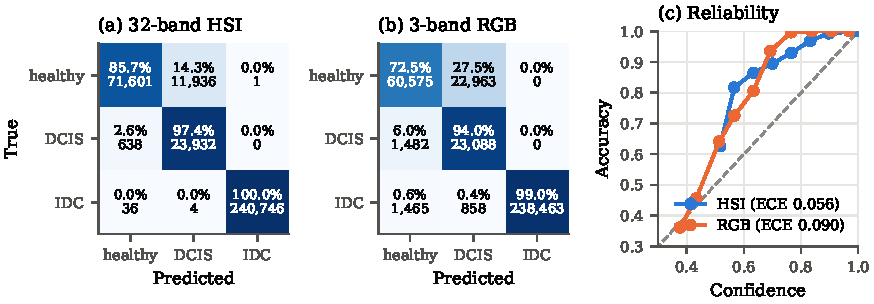
\includegraphics[width=\linewidth]{fig_error_analysis}
\caption{(a, b) Row-normalized test confusion matrices, seed 42. (c) Reliability diagram, 15 bins}
\label{fig:error}
\end{figure}

Training loss falls steadily for both inputs (32 bands: 0.128 to 0.034), while the validation loss of the 32-band model reaches its minimum at epoch 9 (0.101) and rises to 0.169 at epoch 20; validation macro-F1 peaks at epoch 7, and at epoch 4 for the 3-band model (Fig.~\ref{fig:learning}). In a t-SNE~\cite{tsne} of the pooled answer state (Fig.~\ref{fig:tsne}) the three classes form separate groups with 32 bands, whereas with 3 bands healthy and DCIS patches intermix, in agreement with the higher healthy-to-DCIS confusion of the 3-band arm; t-SNE geometry is not a measure of separability.

\begin{figure}[!htb]
\centering
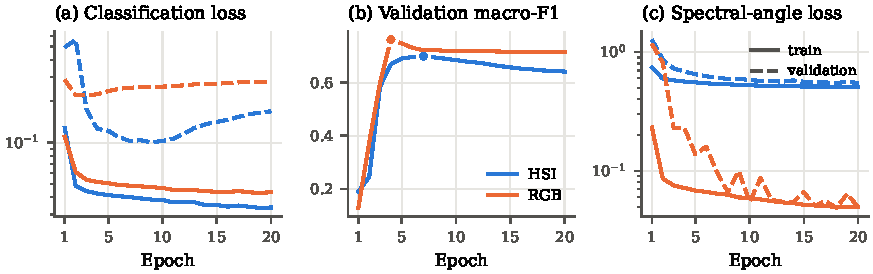
\includegraphics[width=\linewidth]{fig_learning_curves}
\caption{Training dynamics at seed 42: (a) classification loss, (b) validation macro-F1, (c) spectral-angle loss}
\label{fig:learning}
\end{figure}

\begin{figure}[!htb]
\centering
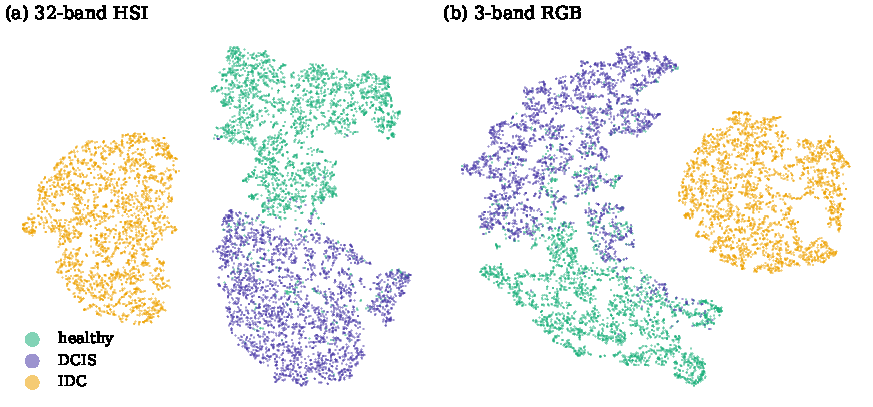
\includegraphics[width=\linewidth]{fig_tsne}
\caption{t-SNE of the pooled answer state, 9,000 class-stratified test patches: (a) 32 bands, (b) 3 bands}
\label{fig:tsne}
\end{figure}

On PAD-UFES-20 (Table~\ref{tab:pad}), MedMamba-SS-TRM was trained on a class-undersampled set of 234 images, and its configuration is one of 33 recursive runs whose test scores were recorded; the repeat of the MedMamba-SS run gives BA 38.4\,\% and macro-F1 0.377; averaging patch predictions per image raises MedMamba from 24.8 to 31.4\,\%; and our MedMamba-T run (47.2\,\% accuracy, ROC-AUC 0.714) is below the 58.8\,\% and 0.808 listed in the MedMamba repository~\cite{medmamba_repo}.

\begin{table}[!htb]
\caption{Whole-image PAD-UFES-20, test split (single runs; bold: best of three)}
\label{tab:pad}
\centering\scriptsize
\begin{tabular}{@{}lrrr@{}}
\toprule
 & MedMamba-SS-TRM & MedMamba-SS & MedMamba-T~\cite{medmamba_repo} \\
\midrule
Parameters & \textbf{0.45\,M} & 27.4\,M & 14.5\,M \\
Split; training / test images & patient; 234 / 344 & patient; 1,626 / 344 & image; 1,378 / 691 \\
Loss & focal, $w \propto n_k^{-1}$ & focal, $w \propto n_k^{-0.75}$ & cross-entropy \\
Accuracy / BA (\%) & 45.6 / \textbf{50.2} & \textbf{53.5} / 39.8 & 47.2 / 33.9 \\
Macro precision / specificity (\%) & \textbf{40.3} / 88.6 & 37.5 / \textbf{89.2} & 34.5 / 87.9 \\
Macro-F1 / Cohen's $\kappa$ & \textbf{0.421} / 0.305 & 0.385 / \textbf{0.352} & 0.335 / 0.271 \\
Macro ROC-AUC & 0.793 & \textbf{0.798} & 0.714 \\
\bottomrule
\end{tabular}
\end{table}

\begin{table}[!htb]
\caption{HistologyHSI-BC-Recurrence: patients / captures / patches per class and split}
\label{tab:split}
\centering\scriptsize
\begin{tabular}{@{}lrrrr@{}}
\toprule
Split & Healthy & DCIS & IDC & All \\
\midrule
Training & 30 / 147 / 722,358 & 5 / 25 / 122,850 & 34 / 327 / 1,606,878 & 35 / 499 / 2,452,086 \\
Validation & 4 / 20 / 98,280 & 1 / 5 / 24,570 & 5 / 49 / 211,666 & 5 / 74 / 334,516 \\
Test & 4 / 17 / 83,538 & 1 / 5 / 24,570 & 5 / 49 / 240,786 & 5 / 71 / 348,894 \\
\bottomrule
\end{tabular}
\end{table}


\emph{MedMamba-SS diagnostics.} On a class-stratified sample of 9,000 test patches (3,000 per class, batches in random order), the standard hierarchical variant in evaluation mode predicts IDC for 8,994 patches (BA 0.334); with batch normalization using each test batch's statistics BA rises to 0.490 (0.487 in training mode), and its running channel means differ from the test batches' by up to 3.8 running standard deviations. For the full-channel variant evaluation mode makes no difference (0.405, 0.388, 0.405). Lowering the learning rate to $10^{-4}$ or $3 \times 10^{-5}$, removing the reconstruction decoder and raising the clipping threshold to 5.0 all leave both variants at chance.

The band gate peaks at 577~nm for DCIS (0.67), then IDC (0.65) and healthy tissue (0.61), although the $\pm$1 s.d.\ bands overlap; at 535~nm healthy tissue reflects 0.17 above the overall mean and DCIS 0.15 below it (Fig.~\ref{fig:xai}). The 32 bands the gate weights were themselves chosen with labels.

\begin{figure}[!htb]
\centering
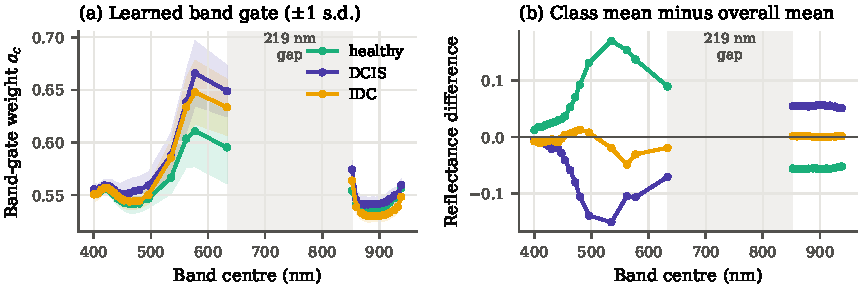
\includegraphics[width=0.92\linewidth]{fig_xai_bands}
\caption{(a) Band-gate weights, 9,000 class-stratified test patches. (b) Each class's mean spectrum minus the overall mean}
\label{fig:xai}
\end{figure}


\subsection{Reproducibility, Data and Use of Generative AI}
Both proposed models are defined in one implementation and selected by one configuration switch. Every run records its configuration, per-epoch history, gate reports, per-patient metrics, arithmetic counts and a checkpoint-reproducibility record; data preparation records its command line, the selected band indices, the per-capture gains and the patient split. Runs are not bitwise deterministic (Sect.~\ref{sec:setup}). HistologyHSI-BC-Recurrence~\cite{hsibc_data,hsibc_desc} (via The Cancer Imaging Archive) and PAD-UFES-20~\cite{pad_desc,pad_data} are used under CC BY 4.0; the MedMamba baseline uses its reference implementation~\cite{medmamba_repo}, and TRM's reference implementation is public~\cite{trm_repo}. Code and checkpoints will be released on acceptance. A generative AI assistant was used to help draft and revise the text and to help write and debug code for the experiments, analyses and figures; the authors directed this work, checked the text, numbers and references against the experimental records, and take full responsibility for the content.

\FloatBarrier
%======================================================================
% ---- Bibliography (order of first citation; build_bibliography.py) ----
%======================================================================
%BIB-BEGIN
\begin{thebibliography}{57}

\bibitem{medmamba}
Yue, Y., Li, Z.: MedMamba: Vision Mamba for medical image classification. arXiv:2403.03849 (2024)

\bibitem{trm}
Jolicoeur-Martineau, A.: Less is more: recursive reasoning with tiny networks. arXiv:2510.04871 (2025)

\bibitem{lu2014}
Lu, G., Fei, B.: Medical hyperspectral imaging: a review. J. Biomed. Opt. \textbf{19}(1), 010901 (2014). \url{https://doi.org/10.1117/1.JBO.19.1.010901}

\bibitem{pandey2026}
Pandey, A., Ahmed, S.B.: Hyperspectral melanoma segmentation using SLIC-derived pseudo-labels. In: Proceedings of the Computer Vision Conference (CVC) 2026, Vol.~3. LNNS, pp. 171--183. Springer, Cham (2026). \url{https://doi.org/10.1007/978-3-032-26217-2_14}

\bibitem{fatima2025}
Fatima, S., Akram, M.U., Mohammad, S., Ahmed, S.B.: Deep learning in dermatopathology: applications for skin disease diagnosis and classification. Discover Appl. Sci. \textbf{7}, 1006 (2025). \url{https://doi.org/10.1007/s42452-025-07138-3}

\bibitem{channelvit}
Bao, Y., Sivanandan, S., Karaletsos, T.: Channel vision transformers: an image is worth 1\,$\times$\,16\,$\times$\,16 words. In: International Conference on Learning Representations (ICLR) (2024). \url{https://openreview.net/forum?id=CK5Hfb5hBG}

\bibitem{dofa}
Xiong, Z., et al.: Neural plasticity-inspired multimodal foundation model for Earth observation. arXiv:2403.15356 (2024)

\bibitem{batformer}
Shahi, N.J., Ahmed, S.B.: Band-aware transformer (BAT-Former) for general image understanding. In: Proceedings of the Computer Vision Conference (CVC) 2026, Vol.~3. LNNS, pp. 184--200. Springer, Cham (2026). \url{https://doi.org/10.1007/978-3-032-26217-2_15}

\bibitem{carl}
Baumann, A., Ayala, L., Seidlitz, S., Sellner, J., Studier-Fischer, A., \"{O}zdemir, B., et al.: CARL: camera-agnostic representation learning for spectral image analysis. arXiv:2504.19223 (2025)

\bibitem{film}
Perez, E., Strub, F., de~Vries, H., Dumoulin, V., Courville, A.: FiLM: visual reasoning with a general conditioning layer. In: Proceedings of the AAAI Conference on Artificial Intelligence, vol.~32 (2018). \url{https://doi.org/10.1609/aaai.v32i1.11671}

\bibitem{resnet}
He, K., Zhang, X., Ren, S., Sun, J.: Deep residual learning for image recognition. In: IEEE Conference on Computer Vision and Pattern Recognition (CVPR), pp. 770--778 (2016). \url{https://doi.org/10.1109/CVPR.2016.90}

\bibitem{convnext}
Liu, Z., Mao, H., Wu, C.-Y., Feichtenhofer, C., Darrell, T., Xie, S.: A ConvNet for the 2020s. In: IEEE/CVF Conference on Computer Vision and Pattern Recognition (CVPR), pp. 11966--11976 (2022). \url{https://doi.org/10.1109/CVPR52688.2022.01167}

\bibitem{vit}
Dosovitskiy, A., et al.: An image is worth 16\,$\times$\,16 words: Transformers for image recognition at scale. In: International Conference on Learning Representations (ICLR) (2021). \url{https://openreview.net/forum?id=YicbFdNTTy}

\bibitem{swin}
Liu, Z., et al.: Swin Transformer: hierarchical vision transformer using shifted windows. In: IEEE/CVF International Conference on Computer Vision (ICCV), pp. 9992--10002 (2021). \url{https://doi.org/10.1109/ICCV48922.2021.00986}

\bibitem{mamba}
Gu, A., Dao, T.: Mamba: linear-time sequence modeling with selective state spaces. In: Conference on Language Modeling (COLM) (2024). \url{https://openreview.net/forum?id=tEYskw1VY2}

\bibitem{vim}
Zhu, L., et al.: Vision Mamba: efficient visual representation learning with bidirectional state space model. In: International Conference on Machine Learning (ICML). PMLR, vol.~235, pp. 62429--62442 (2024)

\bibitem{vmamba}
Liu, Y., et al.: VMamba: visual state space model. In: Advances in Neural Information Processing Systems (NeurIPS), vol.~37, pp. 103031--103063 (2024)

\bibitem{khan2026}
Khan, M.S., Atoofian, E., Ahmed, S.B.: Quantum enchanced [sic] multi-scale CNN with bi-directional Mamba for crop field analysis. arXiv:2606.17222 (2026)

\bibitem{melanospec}
Zhao, Q., Lei, S., Tian, C., Li, W.: Patient-level hyperspectral state-space learning for melanoma pathology diagnosis. Photodiagnosis Photodyn. Ther. \textbf{61}, 105642 (2026). \url{https://doi.org/10.1016/j.pdpdt.2026.105642}

\bibitem{ut}
Dehghani, M., Gouws, S., Vinyals, O., Uszkoreit, J., Kaiser, \L.: Universal Transformers. In: International Conference on Learning Representations (ICLR) (2019). \url{https://openreview.net/forum?id=HyzdRiR9Y7}

\bibitem{albert}
Lan, Z., Chen, M., Goodman, S., Gimpel, K., Sharma, P., Soricut, R.: ALBERT: a lite BERT for self-supervised learning of language representations. In: International Conference on Learning Representations (ICLR) (2020). \url{https://openreview.net/forum?id=H1eA7AEtvS}

\bibitem{deq}
Bai, S., Kolter, J.Z., Koltun, V.: Deep equilibrium models. In: Advances in Neural Information Processing Systems (NeurIPS), vol.~32 (2019)

\bibitem{act}
Graves, A.: Adaptive computation time for recurrent neural networks. arXiv:1603.08983 (2016)

\bibitem{hrm}
Wang, G., et al.: Hierarchical reasoning model. arXiv:2506.21734 (2025)

\bibitem{hybridsn}
Roy, S.K., Krishna, G., Dubey, S.R., Chaudhuri, B.B.: HybridSN: exploring 3-D--2-D CNN feature hierarchy for hyperspectral image classification. IEEE Geosci. Remote Sens. Lett. \textbf{17}(2), 277--281 (2020). \url{https://doi.org/10.1109/LGRS.2019.2918719}

\bibitem{spectralformer}
Hong, D., et al.: SpectralFormer: rethinking hyperspectral image classification with Transformers. IEEE Trans. Geosci. Remote Sens. \textbf{60}, 5518615 (2022). \url{https://doi.org/10.1109/TGRS.2021.3130716}

\bibitem{quantformer}
Ahmed, S.B., Lunia, J.: QuantFormer: a hybrid quantum classical transformer for hyperspectral image classification. In: Proceedings of the 39th Canadian Conference on Artificial Intelligence. PMLR, vol.~318, pp. 103--114 (2026)

\bibitem{fatima2026}
Fatima, S., Salam, A.A., Akram, M.U., Hameed, I.A., Ahmed, S.B.: Incremental learning approach for semantic segmentation of skin histology images. Sci. Rep. \textbf{16}, 9593 (2026). \url{https://doi.org/10.1038/s41598-025-31553-6}

\bibitem{ortega2020gbm}
Ortega, S., Halicek, M., Fabelo, H., Camacho, R., de~la Luz Plaza, M., Godtliebsen, F., et al.: Hyperspectral imaging for the detection of glioblastoma tumor cells in H\&E slides using convolutional neural networks. Sensors \textbf{20}(7), 1911 (2020). \url{https://doi.org/10.3390/s20071911}

\bibitem{ortega2020breast}
Ortega, S., Halicek, M., Fabelo, H., Guerra, R., Lopez, C., Lejaune, M., et al.: Hyperspectral imaging and deep learning for the detection of breast cancer cells in digitized histological images. In: Medical Imaging 2020: Digital Pathology. Proc. SPIE, vol.~11320, 113200V (2020). \url{https://doi.org/10.1117/12.2548609}

\bibitem{spectralgpt}
Hong, D., et al.: SpectralGPT: spectral remote sensing foundation model. IEEE Trans. Pattern Anal. Mach. Intell. \textbf{46}(8), 5227--5244 (2024). \url{https://doi.org/10.1109/TPAMI.2024.3362475}

\bibitem{hypersigma}
Wang, D., et al.: HyperSIGMA: hyperspectral intelligence comprehension foundation model. IEEE Trans. Pattern Anal. Mach. Intell. \textbf{47}(8), 6427--6444 (2025). \url{https://doi.org/10.1109/TPAMI.2025.3557581}

\bibitem{hsibc_data}
Quintana Quintana, L., et al.: Recurrent breast cancer: histopathological and hyperspectral images database (HistologyHSI-BC-Recurrence), version~1 [data set]. The Cancer Imaging Archive (2025). \url{https://doi.org/10.7937/6KPY-YT49}

\bibitem{hsibc_desc}
Quintana-Quintana, L., et al.: Histological hyperspectral breast cancer recurrence database (HistologyHSI-BC Recurrence). Sci. Data \textbf{12}, 1886 (2025). \url{https://doi.org/10.1038/s41597-025-06157-4}

\bibitem{sklearn}
Pedregosa, F., et al.: Scikit-learn: machine learning in Python. J. Mach. Learn. Res. \textbf{12}, 2825--2830 (2011)

\bibitem{pad_desc}
Pacheco, A.G.C., et al.: PAD-UFES-20: a skin lesion dataset composed of patient data and clinical images collected from smartphones. Data Brief \textbf{32}, 106221 (2020). \url{https://doi.org/10.1016/j.dib.2020.106221}

\bibitem{pad_data}
Pacheco, A.G.C., et al.: PAD-UFES-20: a skin lesion dataset composed of patient data and clinical images collected from smartphones, version~1 [data set]. Mendeley Data (2020). \url{https://doi.org/10.17632/zr7vgbcyr2.1}

\bibitem{glu}
Shazeer, N.: GLU variants improve Transformer. arXiv:2002.05202 (2020)

\bibitem{rmsnorm}
Zhang, B., Sennrich, R.: Root mean square layer normalization. In: Advances in Neural Information Processing Systems (NeurIPS), vol.~32 (2019)

\bibitem{senet}
Hu, J., Shen, L., Sun, G.: Squeeze-and-excitation networks. In: IEEE/CVF Conference on Computer Vision and Pattern Recognition (CVPR), pp. 7132--7141 (2018). \url{https://doi.org/10.1109/CVPR.2018.00745}

\bibitem{layerscale}
Touvron, H., Cord, M., Sablayrolles, A., Synnaeve, G., J\'{e}gou, H.: Going deeper with image transformers. In: IEEE/CVF International Conference on Computer Vision (ICCV), pp. 32--42 (2021). \url{https://doi.org/10.1109/ICCV48922.2021.00010}

\bibitem{checkpointing}
Chen, T., Xu, B., Zhang, C., Guestrin, C.: Training deep nets with sublinear memory cost. arXiv:1604.06174 (2016)

\bibitem{focal}
Lin, T.-Y., Goyal, P., Girshick, R., He, K., Doll\'{a}r, P.: Focal loss for dense object detection. In: IEEE International Conference on Computer Vision (ICCV), pp. 2999--3007 (2017). \url{https://doi.org/10.1109/ICCV.2017.324}

\bibitem{naeini}
Naeini, M.P., Cooper, G., Hauskrecht, M.: Obtaining well calibrated probabilities using Bayesian binning. In: Proceedings of the AAAI Conference on Artificial Intelligence, vol.~29, pp. 2901--2907 (2015). \url{https://doi.org/10.1609/aaai.v29i1.9602}

\bibitem{guo2017}
Guo, C., Pleiss, G., Sun, Y., Weinberger, K.Q.: On calibration of modern neural networks. In: International Conference on Machine Learning (ICML). PMLR, vol.~70, pp. 1321--1330 (2017)

\bibitem{brier}
Brier, G.W.: Verification of forecasts expressed in terms of probability. Mon. Weather Rev. \textbf{78}(1), 1--3 (1950). \url{https://doi.org/10.1175/1520-0493(1950)078<0001:VOFEIT>2.0.CO;2}

\bibitem{pytorch}
Paszke, A., et al.: PyTorch: an imperative style, high-performance deep learning library. In: Advances in Neural Information Processing Systems (NeurIPS), vol.~32, pp. 8024--8035 (2019)

\bibitem{adamw}
Loshchilov, I., Hutter, F.: Decoupled weight decay regularization. In: International Conference on Learning Representations (ICLR) (2019). \url{https://openreview.net/forum?id=Bkg6RiCqY7}

\bibitem{ilse}
Ilse, M., Tomczak, J.M., Welling, M.: Attention-based deep multiple instance learning. In: International Conference on Machine Learning (ICML). PMLR, vol.~80, pp. 2127--2136 (2018)

\bibitem{elmore}
Elmore, J.G., et al.: Diagnostic concordance among pathologists interpreting breast biopsy specimens. JAMA \textbf{313}(11), 1122--1132 (2015). \url{https://doi.org/10.1001/jama.2015.1405}

\bibitem{hmilusc}
Yan, Z., Huang, H., Guo, Y., Shi, J., Geng, R., Zhang, J., et al.: HMI-LUSC: a histological hyperspectral imaging dataset for lung squamous cell carcinoma. Sci. Data \textbf{13}, 415 (2026). \url{https://doi.org/10.1038/s41597-026-06766-7}

\bibitem{geifman2017}
Geifman, Y., El-Yaniv, R.: Selective classification for deep neural networks. In: Advances in Neural Information Processing Systems (NeurIPS), vol.~30, pp. 4878--4887 (2017)

\bibitem{medformer}
Sibhai, M.M., Alkhateeb, A., Ahmed, S.B.: MedFormer-UR: uncertainty-routed transformer for medical image classification. arXiv:2604.08868 (2026)

\bibitem{aurc}
Geifman, Y., Uziel, G., El-Yaniv, R.: Bias-reduced uncertainty estimation for deep neural classifiers. In: International Conference on Learning Representations (ICLR) (2019). \url{https://openreview.net/forum?id=SJfb5jCqKm}

\bibitem{tsne}
van~der Maaten, L., Hinton, G.: Visualizing data using t-SNE. J. Mach. Learn. Res. \textbf{9}, 2579--2605 (2008)

\bibitem{medmamba_repo}
Yue, Y., Li, Z.: MedMamba. GitHub repository (2024). \url{https://github.com/YubiaoYue/MedMamba}

\bibitem{trm_repo}
Jolicoeur-Martineau, A.: TinyRecursiveModels. GitHub repository (2025). \url{https://github.com/SamsungSAILMontreal/TinyRecursiveModels}

\end{thebibliography}
%BIB-END
\end{document}
